%!TEX root = ../thesis.tex
%*******************************************************************************
%****************************** Second Chapter *********************************
%*******************************************************************************

\chapter{Branch-and-price for coding-aware routing in wireless networks}
\label{chap.bp}


\section{Introduction}
 \raggedbottom
 
Multi-hop wireless sensor networks (WSNs) support many applications requiring wireless communication on various platforms. We can mention unmanned aerials vehicles (UAVs) \cite{ mozaffari2019tutorial, oubbati2019routing}, flying taxis (Vertical Take-Off and Landing) \cite{pelegrin:hal-02902566}, Internet-of-Things (IoT) sensor devices for monitoring \cite{deebak2020hybrid,wu2019internet}, connected healthcare \cite{gope2015bsn, IoTHealthCare2017}, agricultural monitoring and various emerging smart city and smart mobility deployments \cite{lu2017collaborative,yaqoob2017enabling}, whose components are connected via WSNs. In all these cases, energy efficiency and traffic optimization are key challenges. In the upcoming IoT landscape \cite{akpakwu2017survey, rahimi2018novel}, smart devices are expected to be widely deployed everywhere over the world \cite{fysarakis2016iot}. Current statistics indicate that billions of IoT devices are already deployed and connected in 2020, and they are expected to grow substantially in the future \cite{almeida2020proposal}. 
WSNs are having significant and growing effects on energy consumption and environmental issues. The research community faces solving optimization problems that will shape the connectivity of billions of devices with significant energy issues. 
Most WSN technologies and deployments rely on single-hop communications. Multi-hop communication in WSNs would increase network capacity and coverage without requiring new infrastructure. Extensions to multi-hop communication especially in IoT-related technologies are attracting research and industrial interest \cite{gomez2006adapting,shaikh2018routing}. 

In this chapter, we study the problem of energy efficiency in multi-hop WSNs, namely wireless unsplittable multi-commodity flow with network coding (wUMCFC). We use the DW relaxation for the resulting MILP problem and propose an exact branch-and-price algorithm.

The lifetime of the network strongly depends on the energy level of its devices. Each node in the WSN has limited wireless communication capabilities and energy source (usually a battery). Due to the small sizes of the sensors, the batteries are also small and the available energy is limited. The optimal management of energy is necessary to ensure a long network lifetime. A classification of the main used batteries in the WSN is given in \cite{tiliute2007battery}.

\textbf{Routing strategies} have a major impact on the total energy consumption of networks. In multi-hop WSNs each communication is routed through a single path, i.e., unsplittably from its source node to its target node \cite{baccelli2009,baccelli2010optimization, baccelli2010ospf}. Hence the intermediate nodes in the path are not in charge of computing, for each data packet, the next hop-node.

\textbf{Unsplittable routing} allows intermediate nodes to use less memory, speeds up packet handling processes, minimizes loss rates and enables better quality of service (QoS). However unsplittable routing induces very complex combinatorial optimization problems \cite{barnhart1998branch,BelaidouniB07, kleinberg1996single,vanier2018partition}. Splittable routing is very complex to apply in a wireless context. This would require sophisticated protocols and more intelligence in the network components. For more details on routing protocols in WSNs, we refer to \cite{cordero2011link}.

\textbf{Network coding} allows intermediate nodes of the network to encode several packets into a single packet, and then broadcast, i.e., transmit simultaneously to all neighbours only once \cite{nguyen2008wireless}. Broadcasting is the term used to describe communication where the data packets are sent from one node to all other connected nodes; a single sender transmits data, and the data is sent to all connected receivers. 
Network coding reduces energy consumption in WSNs by reducing the number of transmissions required in a network to carry traffic between the set of sources and the set of destinations \cite{abdul2017efficient, rhaiem2017information, cheng2019high,  jacquet2001optimized, li2003linear}.
The deployment of network coding and broadcasting realizes significant benefits in terms of resource and energy management and improves a network's throughput, efficiency and scalability, as well as resilience to attacks and eavesdropping \cite{Fragouli2008}.

\textbf{Interference} has a significant impact on energy consumption, networking operation and performance. Wireless communication relies on shared communication media, that can be accessed by several devices, close to each other, at the same time. Interference is caused by simultaneous transmissions between these devices. 
Several strategies and models are developed in the literature to handle interference in WSNs \cite{xin2011interference}.


\subsection{Literature review}
In \cite{ni2006routing}, the authors proposed a linear programming model to compute optimal routing, that minimizes the number of data transmissions, without taking into account the interference. In \cite{laube2016optimal}, a MILP was proposed to optimize the routing with network coding, but the effect of energy saved by network coding was not considered.

This article presents mathematical formulations of the wUMCFC problem that integrate interference and network coding. A column generation approach and a branch-and-price framework are then described.
The proposed models are based on the unsplittable multi-commodity flow (UMCF) problem formulations. UMCF is  one of the well-known \(\mathcal{NP}\)-hard problems in combinatorial optimization \cite{atamturk2002splittable,dinitz1999single,kleinberg1996single, kleinberg1998decision}. The problem addressed in this chapter is more complex since it generalizes the UMCF problem with additional coding and interference constraints. Extensive research is required to adapt mathematical programming approaches and develop efficient algorithms to solve it.
Multi-commodity flow models are developed for several network optimization problems since they lead to modeling complex technical constraints \cite{alvarez2012models, bauguion2018maximum, ben2007acceleration, gendron2019revisiting, leitner2020exact, vanier2018partition}. The technical constraints can be the unsplittable routing or resource sharing constraints \cite{atamturk2002splittable, kleinberg1998decision, haddad2019virtual}.
Another advantage of the multi-commodity flow formulations is that they can be solved efficiently by decomposition and column generation methods \cite{barnhart1998branch,gendron2014branch,haddad2019virtual,lubbecke2005selected, pessoa2018automation,vanier2018column}.

\subsection{Contribution}
 The first contribution of this chapter is our quantitative analysis and modelling of interference, network coding and energy consumption in the context of WSNs. We propose the new problem wUMCFC and new models to integrate interference and network coding.
Given the network topology, source-target traffic demands, transmissions capacities, and channels' interference, the wUMCFC problem seeks to minimize the energy cost of data transmission in multi-hop WSNs and find an optimal unsplittable routing. The wUMCFC problem incorporates network coding to reduce data transmission, save energy consumption and improve quality of service (QoS). Interference is modelled using adapted capacity constraints, which are defined over the clique set of an undirected conflict graph.
We show that the wUMCFC problem is an $\mathcal{NP}-$hard problem.

 The second contribution involves our formulations of the  wUMCFC problem. The first class of models are compact edge-based formulations, which consist of a mixed-Boolean quadratic programming (MBQP) formulation and two MILP formulations. The two MILP models are respectively the edge balance formulation and the edge linearization formulation. We study the strength of these two MILP formulations.
 The second class of models is a DW reformulation of the edge balance model, namely a path-based formulation.
 
 
To solve the path-based formulation efficiently, we develop a column generation approach and a branch-and-price (B\(\&\)P) algorithm \cite{alvelos2003comparing, barnhart1998branch, gendron2014branch}. The algorithm is implemented in a new open source solver \textit{wUMCFC}. This yields our third contribution. 
In our B\(\&\)P algorithm, the pricing problem is reduced to a shortest path problem in an extended graph.
Although the edge weights of the extended graph can be negative, we prove that the cycles of the extended graph have positive costs. Therefore, a shortest path in the extended graph can be calculated in polynomial time. We show that, under our reduction, the path generated in the original graph is always a simple path.
We perform a computational study on realistic problem instances with an analysis of the performance of the B\(\&\)P algorithm and the effect of the network coding.

\subsection{Outline the chapter}

This article is organized as follows: In Section \ref{sec1}, we introduce the classical UMCF problem formulation and notation.
We present the three important aspects of the wUMCFC problem: energy consumption, clique capacity constraints and network coding. We then analyze the complexity of the wUMCFC problem.
In Section \ref{sec2}, we present and compare the compact edge-based formulations and the path-based formulation. In Section \ref{sec3}, we propose a new algorithm to solve the LP relaxation of the path-based formulation. We discuss the column generation approach, the pricing problem and the B\(\&\)P algorithm. In Section \ref{sec.branch}, we describe branching rules to enforce the integrality of path variables. In Section \ref{sec5}, we perform two experiments. The first experiment shows that the B\(\&\)P algorithm for the path-based formulation outperforms the MILP solver CPLEX for the edge balance formulation. The second experiment demonstrates that the network coding mechanism can decrease the energy cost significantly. Conclusions are drawn in Section \ref{sec6} along with the prospect of future research.

\section{Models and notation}
\label{sec1}
The network topology is represented by a
bi-directed graph \(G = (V, E)\), where \(V\) denotes the set of nodes corresponding to wireless transmission devices and \(E\) denotes the set of transmission links that can be used to route the traffic.

Unsplittable traffic demands are denoted by a set \( D \) of source-target node pairs \((s,t)\).

We define the following notation of data and parameters:

\(C_{ij}\): the transmission capacity of the edge \( (i,j) \). It measures the number of data packets that can be sent through the channel \((i,j)\) per unit of time.

\(\beta_{ij}\): the energy cost parameter for flow transmission along the edge \((i,j)\). It measures the energy cost to transmit a unit data packet per unit of time.

\(d^{st}\): the traffic demand from the source node \(s\) to the target node \(t\) for \(st \in D\).


\textbf{Decision variables:}

\(x^{st}_{ij}: \) binary variable indicating whether demand \(st\) is routed on the edge \((i,j)\), for $st \in D$ and $(i,j) \in E$.

The occupancy time ratio \textbf{(OTR)} is an important concept in wireless communication. The OTR measures the ratio that the channel along $(i,j)$ is transmitting data per unit of time. Hence, the forwarding node $i$ consumes energies during the transmission time. For each edge $(i,j ) \in E$, its OTR is defined as the total flow per unit of time divided by its capacity, i.e.,
\begin{equation}
    \frac{\sum_{st \in D} d^{st} x^{st}_{ij}}{C_{ij}}.
\end{equation}

The UMCF problem aims to find a unique routing path for each demand that minimizes the total energy cost under capacity and demand constraints.

Before introducing network interference and network coding, let us recall the ILP formulation of the classical minimum cost flow (UMCF) problem:

\begin{equation}\label{MonoNiveau0}
\begin{array}{llll}
\min & z =  \displaystyle \sum_{st \in D} \displaystyle \sum_{(i,j) \in E} \beta_{ij} d^{st} x^{st}_{ij}          &&  (\ref{MonoNiveau0}.0)\\
& \displaystyle \sum_{j:(i,j) \in E} x^{st}_{ij}-\displaystyle \sum_{j:(j,i) \in E} x^{st}_{ji} = 0, & \forall i \in V - \{s,t\},\enspace \forall st \in D, & (\ref{MonoNiveau0}.1)\\
& \displaystyle \sum_{(s, i) \in E} x^{st}_{si} - \displaystyle \sum_{(i, s) \in E} x^{st}_{is}   = 1, & \forall st \in D, & (\ref{MonoNiveau0}.2)\\
& \displaystyle \sum_{(i, t) \in E} x^{st}_{it}  - \displaystyle \sum_{(t, i) \in E} x^{st}_{ti}   = 1, & \forall st \in D, & (\ref{MonoNiveau0}.3)\\
& \displaystyle \sum_{st \in D}  \frac{d^{st}}{C_{ij}}x^{st}_{ij}   \leq 1,  & \forall (i,j) \in E,  & (\ref{MonoNiveau0}.4)\\
& x^{st}_{ij} \in \{0,1\}, &\forall (i,j) \in E, \enspace \forall st \in D.&\\

\end{array}
\end{equation}

\textit{Objective function \(z\) (\ref{MonoNiveau0}.0)}: energy consumption of data transmission per unit of time.

\textit{Flow conservation} constraints (\ref{MonoNiveau0}.1) to (\ref{MonoNiveau0}.3): flow conservation constraints at each node.

\textit{Edge capacity constraint (\ref{MonoNiveau0}.4)}:  the total flow on an edge should not exceed the available transmission capacity. This constraint stipulates that the OTR of an edge must be at most 1.

The mathematical formulation of the wUMCFC problem requires the addition of new constraints and new variables to the classical UMFC. This new problem integrates interference and coding mechanisms.

In the following subsections, we present three important factors of the wUMCFC problem: energy consumption, clique capacity constraints, and network coding. We also analyze the complexity of the wUMCFC problem.


\subsection{Energy consumption}
\label{sec.energy}

This chapter considers the energy consumption induced by data transmissions via active devices in the network.

 A node \(i \in V\) is active when it is transmitting data. We introduce an energy cost parameter \(\beta_{i}\) that measures the cost of energy consumed by an active node \(i\) per unit of time. This parameter depends on the characteristics of the communication device corresponding to the node \(i \).

For \((i,j) \in E\), let \(f_{ij}\) be the flow on the edge, i.e., the number of data packets to transmit from node \(i\) to node \(j\) per unit of time. Recall that the OTR \(\frac{f_{ij}}{C_{ij}}\) is the time ratio that node \(i\) is transmitting data along the channel \((i,j)\). The energy cost per unit of time on the channel \((i,j)\) is \( \frac{f_{ij}}{C_{ij}} \beta_i\). During the remaining part of a time unit \(1-\frac{f_{ij}}{C_{ij}}\), energy is not consumed because the node \(i\) does not transmit data through \((i,j)\). 

The energy cost parameter \(\beta_{ij}\) of \((i,j)\), follows as:
\begin{equation}
    \beta_{ij} = \frac{ \beta_i}{C_{ij}}
\end{equation}

\subsection{Clique capacity constraint}
\label{sec1.sub1}
   The difference between wireless and wired networks lies mainly in the use of communication channels and transmission technologies \cite{yang2005}. In wired networks, the capacity of one channel is not affected by the data transmissions of any other channels. In WSNs, channels inherently share the same communication space, and the interference between channels in a neighborhood would decrease their capacities. When a channel transmits a data packet, it consumes the capacity of its neighbours. Interference reduces transmission capacities significantly \cite{jain2005impact}.  
   
   We model interference using capacity constraints, which are defined over the clique set of an undirected conflict graph \(G_c = (N, L) \) where \(N = E\).
   
  The nodes of the conflict graph \(G_c\) are the edges of the network graph \(G\). The links of \(G_c\) represent interference between the edges of \(G\) which cannot transmit data at the same time.
 
 If two edges in \(G\) are in interference, then a link between their corresponding nodes is added to \(G_c\).
 The graph \(G_c\) is constructed incrementally with an initial empty link set \(L\), as follows:
\begin{enumerate}
    \item \(N = E\) and \(L = \emptyset\).
    \item If \((i,j) \in N \text{ and } (k,l)\in N \) are under interference then \\
      add  the link  \(\left\{(i,j), (k,l)\right\}\) to \( L \): \( L = L \cup \left\{(i,j),  (k,l) \right\}\).
\end{enumerate}

  Interference can be modeled in various ways \cite{gupta2000capacity}. We introduce the \(n-\)dist interference model to construct the conflict graphs in our experiments. The \(n-\)dist model extends single-node and two-node models proposed in \cite{chaporkar2008throughput}.
 
   Let $p=(v_1,\hdots,v_h)$ be a simple path in the graph $G$, where $v_t$ ( $t \in \{1,\hdots,h\}$) is the node in the path $p$. We define the length of $p$ as the number of nodes $h$ in the path. For $i,k \in V$, we define $\textrm{dist}(i,k)$ as the length of a shortest path from $i$ to $k$ or from $k$ to $i$, i.e., a path with the minimum number of nodes. For \((i,j) \text{ and } (k,l) \in E\), the distance \(\textrm{dist}\left ((i,j), (k,l)\right)\) is defined as the length of a shortest path between any pair of \(\{i, k\}, \{i, l\}, \{j, k\}, \text{and } \{j, l\}\), i.e., $\textrm{dist}\left ((i,j),  (k,l)\right) = \min_{t_1\in\{i,j\},  t_2 \in \{ k,l\}}\{\textrm{dist}(t_1, t_2), \textrm{dist}(t_2, t_1)\}$. Hence, $\textrm{dist}\left ((i,j),  (k,l)\right)$ measures the minimum distance between the tail and end nodes of edges  \((i,j) \text{ and } (k,l)\) .
 
 Under the \(n-\)dist model, \((i,j) \text{ and } (k,l)\) are in interference if \(\textrm{dist}\left ((i,j),  (k,l)\right) \le n\).
 
 
For example, Figure \eqref{figinter.1} shows a network of five nodes and Figure \eqref{figinter.2} shows its conflict graph constructed via the \(2-\)dist interference model. The \(2-\)dist interference model corresponds to the single-node model in \cite{chaporkar2008throughput}. This model considers that a node interferes with its neighbors.  

The distance between (1,2) and  (4,5) is 3, so they are not connected via any link in  \(G_c\).

The distance between  (1,2) and  (3,4) is 2, so they are connected via one link in  \(G_c\). 
If two edges in \(G\) are in interference, then a link between their corresponding nodes is in \(G_c\).
Hence we can check whether two edges share capacity by the adjacency of their corresponding nodes in \(G_c\).

\begin{figure}[htbp]
\centering
\subfloat[Network with 5 nodes]{
  \begin{tikzpicture}[
    mycircle/.style={
    circle,
    draw=black,
    fill=gray,
    fill opacity = 0.3,
    text opacity=1,
    inner sep=0pt,
    minimum size=12pt,
    font=\small},
    myarrow/.style={-Stealth,font=\small},
    node distance=0.3cm and 0.3cm
    ]
    \node[mycircle] (c1) {$1$};
    \node[mycircle, below right = of c1] (c2) {$2$};
    \node[mycircle, below right= of c2] (c3) {$3$};
    \node[mycircle, below right= of c3] (c4) {$4$};
    \node[mycircle, below right = of c4] (c5) {$5$};

    \draw[myarrow] (c1.315) -- (c2.135);
    \draw[myarrow] (c2.315) -- (c3.135);
    \draw[myarrow] (c3.315) -- (c4.135);
    \draw[myarrow] (c4.315) -- (c5.135);
    \draw[myarrow] (c5.135) -- (c4.315);
\end{tikzpicture}
    \label{figinter.1}
}
\qquad \qquad \qquad \qquad \qquad
\subfloat[Conflict graph]{
      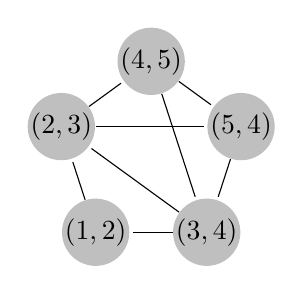
\begin{tikzpicture}[shorten >=1.1pt,-]
  \tikzstyle{node}=[circle,fill=black!25,minimum size=2pt,inner sep=0pt, myarrow/.style={-Stealth,font=\footnotesize}]

  \foreach \name/\angle/\text in {P-1/234/{(1,2)}, P-2/162/{(2,3)},
                                  P-3/90/{(4,5)}, P-4/18/{(5,4)}, P-5/-54/{(3,4)}}
    \node[node,xshift=10cm,yshift=1.2cm] (\name) at (\angle:1.2cm) {$\text$};
  \foreach \from/\to in {1/2,2/3,3/4,4/5,5/1,2/4,3/5,5/2}
    { \draw (P-\from) -- (P-\to); }
\end{tikzpicture}    \label{figinter.2}}
\caption{Interference model}
\label{figinter}
\end{figure}
We develop a capacity-sharing model in a wireless communication context from \cite{gupta2007sufficient}.

 For edge \((i,j) \in E\), let \(f_{ij}\) be the flow on this edge; recall that \(\frac{f_{ij}}{C_{ij}}\) is the OTR of this edge. Two edges connected in the conflict graph cannot transmit at the same time otherwise these transmissions will fail.

Let \(m\) be a subset of edges of \(G\) such that the corresponding nodes in \(G_c\) are a clique. Then every edge of \(m\) shares OTR with other edges in \(m\).

The sum of  OTRs of edges in \(m\) should be at most 1 and the clique capacity constraint follows as:
 
\begin{equation}\sum_{(i,j) \in m}\frac{f_{ij}}{C_{ij}} \le 1.
\end{equation}

 For any two clique sets \(m_1 \) and \(m_2\), such that \(m_1 \subset m_2\), it follows that the clique capacity constraint over \(m_1\) is dominated by the clique capacity constraint over \(m_2\):  

\begin{equation}\sum_{(i,j) \in m_1}\frac{f_{ij}}{C_{ij}} \le \sum_{(i,j) \in m_2}\frac{f_{ij}}{C_{ij}}.
\end{equation}

Therefore, non-dominated constraints are defined over maximal cliques. The dominance relation over clique capacity constraints is equivalent to set inclusion over the corresponding cliques. Then, it suffices to consider only non-dominated constraints induced by maximal cliques in the model.  

We denote by \(M\) the set of maximal cliques of \(G_c\).

In Figure \eqref{figinter.2}, \(m_1 = \) \(\left \{(1,2), (2,3) \right\}\) is a clique set, but  \(m_2 =  \)\(\left \{(1,2), (2,3), (3,4)\right\}\) is the maximal clique set including it, therefore the capacity constraint is expressed only on the maximal clique \(m_2\). 

There are two maximal cliques of \(G_c\) in Figure \eqref{figinter.2}, and hence
\begin{equation*}
M = \left\{\left \{ (1,2),(2,3),(3,4) \right\}, \left\{(2,3),(3,4), (4,5), (5,4) \right \} \right\}.
\end{equation*}


The model contains two capacity constraints:

\begin{equation*}
    \begin{split}
        \sum_{(i,j) \in \left \{ (1,2), (2,3), (3,4) \right \}} \frac{f_{ij}}{C_{ij}} &\le 1, \\
        \sum_{(i,j) \in \left \{ (2,3),(3,4), (4,5), (5,4) \right \}} \frac{f_{ij}}{C_{ij}} &\le 1.
    \end{split}
\end{equation*}


The following section is dedicated to presenting the network coding technique in WSN. 

\subsection{Network coding} \label{sec1.subsec2}
Network coding allows intermediate nodes to combine data packets into a single packet before broadcasting. It is a networking technique where operations, which in practice tend to be algebraic algorithms, are performed on data to reduce the number of transmissions and energy consumption.
Broadcasting is the term used to describe communication where the data packets are sent from one node to all other connected nodes.

Figure \eqref{fig1} illustrates the network coding mechanism by a triple of nodes; node \(j \in V\) and node \(k \in V\) send packets \(P_1\) and \(P_2\) to each other through the intermediate node \(i \in V\).
 
 The classical forwarding scheme in Figure \eqref{fig1.1} uses four transmissions to send \(P_1\) and \(P_2\). Node \(j\) (resp. \(k\)) sends its packet \(P_1\) (resp. \(P_2\)) to node \(i\), and node \(i\) sends \(P_1\) to \(k\) and \(P_2\) to \(j\), separately.

Figure \eqref{fig1.2} shows that with network coding, only three transmissions are needed, and hence the energy cost at the device \(i\) is saved. 
First node \(j\) and node \(k\) record and send their packets to node \(i\). Then node \(i\) encodes these two data packets by XOR operation to obtain an encoded packet \(P_3 \coloneqq P_1 \oplus P_2\), where $\oplus$ is the bit-wise Boolean addition. Node \(i\) broadcasts the encoded packet \(P_3\) to  node \(j\) and node \(k\) simultaneously. Finally, node \(j\) and node \(k\) decode data of \(P_3\) by XOR-ing with recorded packets,  \(P_1 = P_3 \oplus P_2\) and \(P_2 = P_3 \oplus P_1\).

\begin{figure}
\centering
\subfloat[Classical forwarding]{
     \begin{tikzpicture}[
    mycircle/.style={
    circle,
    draw=black,
    fill=gray,
    fill opacity = 0.3,
    text opacity=1,
    inner sep=0pt,
    minimum size=12pt,
    font=\small},
    myarrow/.style={-Stealth,font=\small},
    node distance=1.5cm and 1.5cm
    ]
    \node[mycircle] (c1) {$j$};
    \node[mycircle, right= of c1] (c2) {$i$};
    \node[mycircle, right= of c2] (c3) {$k$};

    \draw[myarrow] (c1.-10) -- (c2.190);
    \draw[myarrow] (c2. 170) -- (c1.10);
    \draw[myarrow] (c2.-10) -- (c3.190);
    \draw[myarrow] (c3. 170) -- (c2.10);

    \draw[myarrow] [red] (c2. 170) -- (c1.10) node [midway, above] {{$ P_{2}$}};
    \draw[myarrow] [red] (c3. 170) -- (c2.10) node [midway, above] {{$ P_{2}$}};
    \draw[myarrow] [blue] (c2. -10) -- (c3.190) node [midway, below] {{$ P_{1}$}};
    \draw[myarrow] [blue] (c1. -10) -- (c2.190) node [midway, below] {{$ P_{1}$}};
\end{tikzpicture}     \label{fig1.1}}
\vfill
\subfloat[Forwarding with network coding]{
     \begin{tikzpicture}[
    mycircle/.style={
    circle,
    draw=black,
    fill=gray,
    fill opacity = 0.3,
    text opacity=1,
    inner sep=0pt,
    minimum size=12pt,
    font=\small},
    myarrow/.style={-Stealth,font=\small},
    node distance=1.5cm and 1.5cm
    ]
    \node[mycircle] (c1) {$j$};
    \node[mycircle, right= of c1] (c2) {$i$};
    \node[mycircle, right= of c2] (c3) {$k$};

    \draw[myarrow] (c1.-10) -- (c2.190);
    \draw[myarrow] (c2. 170) -- (c1.10);
    \draw[myarrow] (c2.-10) -- (c3.190);
    \draw[myarrow] (c3. 170) -- (c2.10);

    \draw[myarrow] [green] (c2. 170) -- (c1.10) node [midway, above] {{$ P_3 = P_1 \oplus P_2$}};
    \draw[myarrow] [red] (c3. 170) -- (c2.10) node [midway, above] {{$ P_{2}$}};
    \draw[myarrow] [green] (c2. -10) -- (c3.190) node [midway, below] {{$  P_3 = P_1 \oplus P_2$}};
    \draw[myarrow] [blue] (c1. -10) -- (c2.190) node [midway, below] {{$ P_{1}$}};
\end{tikzpicture}    \label{fig1.2}}
\caption{Network coding}
\label{fig1}
\end{figure}

If \( (j,i),(i,k),(k,i)\), and \((i,j) \) are in \( E\), then there is a coding opportunity on the node \(i\) called the three-node pattern.

The opportunity set is defined as follows:

\begin{equation}
    \Lambda^i_{\{k,j\}} \coloneqq \left \{(j,i),(i,k),(k,i),(i,j)\right \}.
\end{equation}

For \( \Lambda^i_{\{k,j\}} \subset E\), let \(f_{jik}\)  be the flow along  \(j \to i \to k\), and let \(f_{kij}\) be the flow along \(k \to i \to j\). 

If \(f_{jik}\) and \(f_{kij}\) are non-zero, then network coding can be applied, and the node \(i\) could encode the opposite flows \(f_{jik}\) and \(f_{kij}\).  

We define \(u^i_{\{k,j\}}\) as the flow encoded by node \(i\), and it measures the number of data packets in \(f_{jik}\) and \(f_{kij}\) that node \(i\) could code per unit of time.

Since the maximum encoded data cannot exceed the number of data arriving at a node \(i\),  \(u^i_{\{k,j\}}\) must satisfy the following inequality: 

\begin{equation}
\label{codineq}
u^i_{\{k,j\}} \le \min (f_{jik}, f_{kij}).
\end{equation}

 The next sections explain how the network coding increases the capacity of the network and decreases the energy cost.

\subsubsection{Effects on clique capacity constraints}\label{cliqueCapacity}

Network coding decreases the left-hand side of the capacity constraints since it reduces the occupancy time rate (OTR).
Without network coding, the OTRs sum for transmitting \(f_{jik}\) and \(f_{kij}\) is:\\
\begin{equation}
    \frac{f_{jik}}{C_{ji}}+ \frac{f_{jik}}{C_{ik}} +  \frac{f_{kij}}{C_{ki}}+ \frac{f_{kij}}{C_{ij}}.
\end{equation}

Let \(T^i_{\{k,j\}} u^i_{\{k,j\}}\) be the OTR of the broadcasted flow \(u^i_{\{k,j\}}\) by network coding,
where \(T^i_{\{k,j\}}\) is a network transmission parameter.
The broadcasting time must be at least the time of one of the two separate transmissions: 
  
  \begin{equation}
      T^i_{\{k,j\}} \ge \max \{\frac{1}{C_{ik}}, \frac{1}{C_{ij}}\},
  \end{equation}
 
 The remaining parts of \(f_{jik} - u^i_{\{k,j\}}\) and \(f_{kij} - u^i_{\{k,j\}}\) are transmitted by the classical forwarding scheme.
 
  The OTR with network coding follows as:

\begin{equation}
\begin{split}
&\frac{f_{jik}}{C_{ji}}+ \frac{f_{jik}  -  u^i_{\{k,j\}}}{C_{ik}} +  \frac{f_{kij} }{C_{ki}}+ \frac{f_{kij} - u^i_{\{k,j\}}}{C_{ij}} +T^i_{\{k,j\}} u^i_{\{k,j\}} \\
=     & \frac{f_{jik}}{C_{ji}}+ \frac{f_{jik}}{C_{ik}} +  \frac{f_{kij}}{C_{ki}}+ \frac{f_{kij}}{C_{ij}}  - (\frac{1}{C_{ij}}  +\frac{1}{C_{ik}} - T^i_{\{k,j\}}) u^i_{\{k,j\}}.
\end{split}
\end{equation}

Let \(C^i_{\{k,j\}}\) be the increased capacity over the three-node pattern \(\Lambda^i_{\{k,j\}}\) with network coding. \(C^i_{\{k,j\}}\) measures the number of data packets that will no longer be transmitted on \(\Lambda^i_{\{k,j\}}\) due to network coding:

\begin{equation}
 \frac{1}{C^i_{\{k,j\}}} \coloneqq \frac{1}{C_{ij}}  +\frac{1}{C_{ik}} - T^i_{\{k,j\}}.    
\end{equation}

From the bound on \( T^i_{\{k,j\}}\), the following bound on \(\frac{1}{C^i_{\{k,j\}}}\) is obtained:
\begin{equation}
\label{capbound}
\frac{1}{C^i_{\{k,j\}}} \le \min \left \{  \frac{1}{C_{ij}},  \frac{1}{C_{ik}}  \right \}.
\end{equation}
Equivalently, \(C^i_{\{k,j\}} \ge \max \{C_{ij}, C_{ik} \}\).

As a result, the OTR can be rewritten as:

\begin{equation}
 \frac{f_{jik}}{C_{ji}}+ \frac{f_{jik}}{C_{ik}} +  \frac{f_{kij}}{C_{ki}}+ \frac{f_{kij}}{C_{ij}} - \frac{ u^i_{\{k,j\}}}{C^i_{\{k,j\}}}.
\end{equation}
The OTR decrease within \(\Lambda^i_{\{k,j\}}\) is \(\frac{ u^i_{\{k,j\}}}{C^i_{\{k,j\}}} \).

Let $m \in M$  be a maximal clique of $G_c$. The clique capacity constraint is obtained by summing up the OTRs decreased by network coding, for all opportunity sets in \(m\):

\begin{equation}
\label{setcaprev}
\sum_{(i,j) \in m} \frac{f_{ij}}{C_{ij}} - \sum_{  \Lambda^i_{\{k,j\}} \subset m} \frac{ u^i_{\{k,j\}}}{C^i_{\{k,j\}}} \le 1. \end{equation}

Inequalities \eqref{setcaprev} and \eqref{codineq} define the clique capacity constraint with network coding.

 In our experiments, we set \(T^i_{\{k,j\}}\) to its lower bound \(\max \{\frac{1}{C_{ki}}, \frac{1}{C_{ij}}\}\), 
 and correspondingly set $C^i_{\{k,j\}}$ to $1 / ( \frac{1}{C_{ij}}  +\frac{1}{C_{ik}} - T^i_{\{k,j\}}) = \min \{C_{ki}, C_{ij}\}$.
 
 In practice, the OTR of broadcasting \(u^i_{\{k,j\}}\) can be at most equal to the lower bound \(\max  \left \{\frac{u^i_{\{k,j\}}}{C_{ki}}, \frac{u^i_{\{k,j\}}}{C_{ij}} \right \}\); a higher \(C^i_{\{k,j\}}\) can be set accordingly.

 \subsubsection{Effects on energy consumption}
Network coding allows us to reduce the energy cost and decrease the objective function value.

Without network coding, the energy consumption to send the flow \(u^i_{\{k,j\}}\) from node \(i\) to node \(j\) and to node \(k\) separately is \(u^i_{\{k,j\}}(\beta_{ij} + \beta_{ik})\). Let \({\beta}^i_{\{k,j\}} u^i_{\{k,j\}}\) be the cost of broadcasting \(u^i_{\{k,j\}}\) by network coding, where the energy cost parameter \({\beta}^i_{\{k,j\}}\) measures the energy consumption to send a unit packet of  \(u^i_{\{k,j\}}\) per unit time by broadcasting. 
The transmission cost \({\beta}^i_{\{k,j\}} u^i_{\{k,j\}}\) is equal to the OTR of broadcasting \(u^i_{\{k,j\}}\) times \(\beta_i\), i.e., \({\beta}^i_{\{k,j\}} u^i_{\{k,j\}}=u^i_{\{k,j\}}T^i_{\{k,j\}} \beta_i\). Dividing by \(u^i_{\{k,j\}}\), it follows that   \({\beta}^i_{\{k,j\}} = \beta_i T^i_{\{k,j\}}\).

Therefore, the energy cost of sending flow \(f_{jik}\) and \(f_{kij}\) is reduced to
\begin{equation}
\begin{split}
    &\beta_{ji}f_{jik}+ \beta_{ik}(f_{jik}- u^i_{\{k,j\}}) +  \beta_{ki} f_{kij}+ \beta_{ij}(f_{kij} - u^i_{\{k,j\}}) +\beta^i_{\{k,j\}} u^i_{\{k,j\}} \\
    =& \beta_{ji}f_{jik}+ \beta_{ik}f_{jik} +  \beta_{ki} f_{kij}+ \beta_{ij}f_{kij}  - u^i_{\{k,j\}} (\beta_{ik} +\beta_{ij} - \beta^i_{\{k,j\}}  ).
\end{split}
\end{equation}


Denote \(\tau^i_{\{k,j\}} = \beta_{ij} + \beta_{ik} - {\beta}^i_{\{k,j\}}\), so the energy cost saved by network coding is \(\tau^i_{\{k,j\}}u^i_{\{k,j\}}\). The energy saving and the increased capacity are coupled according to Section \ref{sec.energy}:

\begin{equation}
\tau^i_{\{k,j\}} = \beta_{i}\left(\frac{1}{C_{ij}} + \frac{1}{C_{ik}} - T^i_{\{k,j\}}\right) = \beta_i \frac{1}{C^i_{\{k,j\}}}. \end{equation}


It follows from Section \ref{sec.energy} and the inequality \eqref{capbound} that:

\begin{equation}
\label{redbound}
0 \le \tau^i_{\{k,j\}} \le \beta_i \min  \left \{  \frac{1}{C_{ij}},  \frac{1}{C_{ik}}  \right \} \le \min\left \{\beta_{ij}, \beta_{ik}\right\}.
\end{equation}


\subsection{Complexity analysis}
The wUMCFC problem is formulated as an UMCF problem with additional network coding and clique capacity constraints.
 The wUMCFC problem can be reduced to a single-source unsplittable flow problem \cite{dinitz1999single,kleinberg1996single, kleinberg1998decision,martens2007convex} by considering a single source demand, where clique sets are singletons, and the coding variables are fixed to zero.
 
The single-source unsplittable flow problem is \(\mathcal{NP}-\)hard, hence the wUMCFC problem is also \(\mathcal{NP}-\)hard.

\section{Mathematical Formulations} \label{sec2}

In this section, we present mathematical programming formulations of the wUMCFC problem: the compact edge-based formulations and the path-based formulation. We first define the problem notation.

We denote by wUMCF the model derived from the UMCF problem by including network coding variables and constraints. The edge capacity constraints are reformulated as the clique capacity constraints defined in Section \ref{cliqueCapacity}.
 Moreover, the objective function \(z_{-}\) is obtained by subtracting from \(z\) the energy cost saved by network coding \(z_c\); where \(z_c \coloneqq \sum_{\Lambda^i_{\{k,j\}} \subset E}\tau^i_{\{k,j\}}u^i_{\{k,j\}}\). 

An abbreviation for edge (resp. path) formulation, i.e., E$\#$ (resp. P), is appended at the end of the model notation, where $\#$ will be revealed subsequently. For example, wUMCFC-P denotes the path-based formulation of the wUMCFC problem.

\subsection{Compact edge-based formulations}
In this subsection, we propose the MBQP formulation, and derive two edge-based MILP formulations: the edge linearization formulation and the edge balance formulation. 

\subsubsection{MBQP formulation}

The decision variables of the MBQP formulation are defined as follows:


\textbf{Decision variables:}

\(x^{st}_{ij}: \) binary variable indicating whether demand \(st \in D\) is routed on the edge \((i,j) \in E\).

\(q^{st}_{jik}:\) real variable denoting the flow value of the demand \(st \in D\) routed on the incident edges \(j \to i \to k\). \(q^{st}_{jik}\) should satisfy the quadratic constraint: \(q^{st}_{jik} = d^{st} x^{st}_{ji}  x^{st}_{ik}\).

\(u^i_{\{k,j\}}:\) real coding variable denoting the value of two opposite flows along the incident edges \(k \to i \to j\) and \(j \to i \to k\), which would be encoded at the node \(i\). \\


\(M\) is the set of the maximum cliques of the conflict graph \(G_c\), and \(\tau^i_{\{k,j\}}u^i_{\{k,j\}}\) (\(\Lambda^i_{\{k,j\}} \subset E\)) is the energy cost saved by network coding.

The MBQP formulation, denoted by wUMCFC-EQ, follows as:

\begin{equation}
\resizebox{0.91\hsize}{!}{$
\begin{array}{llll}
\min &z_{-} =  \displaystyle \sum_{st \in D} \displaystyle \sum_{(i,j) \in E} \beta_{ij} d^{st} x^{st}_{ij}   -  \displaystyle   \sum_{\Lambda^i_{\{k,j\}} \subset E}   \tau^i_{\{k,j\}}u^i_{\{k,j\}}     &&  (\ref{MonoNiveau4}.0)\\
\displaystyle  & \sum_{(i,j) \in E} x^{st}_{ij}-\displaystyle \sum_{(j,i) \in E} x^{st}_{ji} = 0, & \forall i \in V - \{s,t\},\enspace \forall st \in D, & (\ref{MonoNiveau4}.1)\\
\displaystyle &  \sum_{(s, i) \in E} x^{st}_{si} - \displaystyle \sum_{(i, s) \in E} x^{st}_{is}   = 1, & \forall st \in D, & (\ref{MonoNiveau4}.2)\\
\displaystyle  & \sum_{(i, t) \in E} x^{st}_{it}  - \displaystyle \sum_{(t, i) \in E} x^{st}_{ti}   = 1, & \forall st \in D, & (\ref{MonoNiveau4}.3)\\
& q^{st}_{jik} - d^{st}x^{st}_{ji}x^{st}_{ik} = 0, & \forall (j,i),(i,k) \in E, \enspace \forall st \in D, & (\ref{MonoNiveau4}.4)\\
& u^i_{\{k,j\}} - \displaystyle \sum_{st \in D} q^{st}_{jik} \le 0, &\forall
 \Lambda^i_{\{k,j\}}  \subset E,&(\ref{MonoNiveau4}.5)\\
& u^i_{\{k,j\}} - \displaystyle \sum_{st \in D} q^{st}_{kij} \le 0, &\forall
 \Lambda^i_{\{k,j\}}  \subset E,&(\ref{MonoNiveau4}.6)\\
& \displaystyle \sum_{st \in D} \displaystyle \sum_{(i,j) \in m} \frac{d^{st}}{C_{ij}}x^{st}_{ij}  - \displaystyle \sum_{ \Lambda^i_{\{k,j\}}  \subset m}    \frac{u^i_{\{k,j\}}}{C^i_{\{k,j\}}}   \leq 1,  & \forall m \in M,  & (\ref{MonoNiveau4}.7)\\
& x^{st}_{ij} \in \{0,1\}, &\forall (i,j) \in E, \enspace \forall st \in D,&\\
&  q^{st}_{jik} \in \mathbb{R}_{+}, &\forall (j,i),(i,k) \in E,  \enspace \forall st \in D,&\\
& u^i_{\{k,j\}}  \in \mathbb{R}_{+}, &\forall \Lambda^i_{\{k,j\}} \subset E .&\\
\end{array}
$}
\label{MonoNiveau4}
\end{equation}



\textit{Objective function \(z_{-}\)  (\ref{MonoNiveau4}.0)}: the energy consumption of data transmissions per unit of time, after removing the energy cost saved by network coding.

\textit{Flow conservation constraints (\ref{MonoNiveau4}.1) to (\ref{MonoNiveau4}.3)}: incoming and outgoing flows at each node are balanced. 

\textit{Incident edge flow constraints (\ref{MonoNiveau4}.4)}: the flow $q^{st}_{jik}$ on incident edges $(j,i)$ and $(i,k)$ is equal to $d^{st}$ if the demand $st$ uses an unsplittable path through $(j,i)$ and $(i,k)$, otherwise $q^{st}_{jik} =0$.

\textit{Coding opportunity constraints (\ref{MonoNiveau4}.5) and (\ref{MonoNiveau4}.6)}: the coding variable \(u^i_{\{k,j\}}\) (cf. inequality \eqref{codineq}) is at most the minimum of two opposite aggregated flows along \(j\to i \to k\) and \(k \to i \to j\).

\textit{Clique capacity constraint (\ref{MonoNiveau4}.7)} with network coding: the OTR within the clique set \(m\) should be at most 1 (cf. \eqref{setcaprev}).

The wUMCFC-EQ formulation contains the classical constraints of the UMCF problem, and additional clique capacity constraints, quadratic constraints and network coding constraints and variables. The next section is dedicated to presenting an edge linearization of the wUMCFC-EQ problem.

\subsubsection{Edge linearization formulation}

We propose an MILP reformulation of the nonlinear MBQP formulation.

The constraint \(q^{st}_{jik} = d^{st} x^{st}_{ji}  x^{st}_{ik}\) is quadratic, \( x^{st}_{ji}\) and \( x^{st}_{ik}\) are binary variables, so we propose the exact linearization approach as follows:
\begin{equation}
\label{reflinear}
\begin{split}
    q^{st}_{jik} &\ge d^{st} (1 - x^{st}_{ji} - x^{st}_{ik}),\\
    q^{st}_{jik} &\le d^{st}  x^{st}_{ji}, \\
   q^{st}_{jik} &\le d^{st}  x^{st}_{ik},\\
   q^{st}_{jik} & \ge 0.
\end{split}
\end{equation}

The edge linearization formulation, denoted by wUMCFC-EL,  replaces incident edge flow constraints (\ref{MonoNiveau4}.4) of the wUMCFC-EQ formulation with the following linearization constraints:
\begin{align}
\label{linearcons}
    q^{st}_{jik}& \ge d^{st} (1 - x^{st}_{ji} - x^{st}_{ik}), &  \forall (j,i) \in E, \enspace \forall (i,k) \in E,\enspace \forall st \in D,\\
    q^{st}_{jik} &\le d^{st}  x^{st}_{ji}, & \forall (j,i) \in E, \enspace \forall (i,k) \in E,\enspace \forall st \in D,\\
   q^{st}_{jik} &\le d^{st}  x^{st}_{ik}, & \forall (j,i) \in E, \enspace \forall (i,k) \in E, \enspace\forall st \in D,\\
   q^{st}_{jik} & \ge 0, &  \forall (j,i) \in E, \enspace \forall (i,k) \in E,\enspace \forall st \in D.
\end{align}
Indeed, the wUMCFC-EL is a standard linearization of the wUMCFC-EQ problem, which is currently used by commercial solvers such as CPLEX \cite{bliek1u2014solving}.

\subsubsection{Edge balance formulation}

The edge balance formulation uses the balanced property of flows on edges to represent the flows on incident edges. We denote the edge balance formulation by wUMCFC-EB. More precisely, the wUMCFC-EB formulation replaces incident edge flow constraints (\ref{MonoNiveau4}.4) of the wUMCFC-EQ formulation with the following edge balance constraints:

\begin{equation}
\label{cons.adjedge}
\begin{split}
        \displaystyle\sum_{(i, k) \in E} q^{st}_{jik} - d^{st} x^{st}_{ji} = 0,  \enspace \forall (j,i) \in E, \enspace \forall st \in D,&\\
\displaystyle\sum_{(j, i) \in E} q^{st}_{jik} - d^{st} x^{st}_{ik} = 0,\enspace \forall (i,k) \in E,\enspace \forall st \in D.&
\end{split}
\end{equation}
The wUMCFC-EB is an MILP formulation.

We illustrate the usage of subscript/superscript notation for the subsequent part of this chapter. When we omit subscripts and/or superscripts of some variables, we denote the subset of variables restricted to the remaining subscripts and/or superscripts. For example, $x$ denotes the set of flow variables indexed by entire superscripts (demands) and subscripts (edges), and $x^{st}$ denotes the set of $st-$flow variables indexed by entire subscripts (edges).

The wUMCFC-EB is a reformulation of the wUMCFC-EQ formulation by the following theorem.

\begin{theorem}
Let $x$ take binary values satisfying flow conservation constraints on nodes (\ref{MonoNiveau4}.1), (\ref{MonoNiveau4}.2) and (\ref{MonoNiveau4}.3). Then $q$ satisfies (\ref{MonoNiveau4}.4) if and only if  $q$ satisfies \eqref{cons.adjedge}.
\end{theorem}
\begin{proof}
Assume $x$ takes binary values satisfying flow conservation constraints on nodes (\ref{MonoNiveau4}.1), (\ref{MonoNiveau4}.2) and (\ref{MonoNiveau4}.3). Then, $x$ already represents an UMCF. For any $(j,i)$ and $(i,k) \in E$ and $st \in D$,   \(q^{st}_{jik} = d^{st} x^{st}_{ji}  x^{st}_{ik}\)  if and only if $q^{st}_{jik}$ is the value of binary $st$-flow over incident edges $(j,i)$ and $(i,k)$. For each $st \in D$, since $x^{st}$ is an unsplittable flow, the $st-$flow takes a unique path from $s$ to $t$. Then the latter condition is equivalent to: for any edge $(i,j) \in E$, the $st-$ flow entering $(i,j)$ from its incident edges  equals the $st-$ flow leaving from $(i,j)$ to its incident edges, which is  exactly the edge balance constraint \eqref{cons.adjedge}.
\end{proof}

According to the following theorem, the linear relaxation of the wUMCFC-EL formulation is not stronger than the linear relaxation of the wUMCFC-EB formulation.

\begin{theorem}
The optimal value of the linear relaxation of the wUMCFC-EL formulation is at most the optimal value of the wUMCFC-EB formulation.
\end{theorem}
\begin{proof}
Let \((\bar{x}, \bar{q}, \bar{u})\) be a feasible solution of the linear relaxation of the wUMCFC-EB formulation. Since the $\bar{x}$ of the relaxation represents a fractional MCF, for each \(st \in D\), we can partition \(\bar{x}^{st}\) and \(d^{st}\) into a finite number of unsplittable \(st-\)flows. Denote by \(\chi^{st}\) the set of paths on which \(st-\)flows in the relaxation solution have non-zero values, and let \(I^p_{ij} \in \{0,1\}\) (\((i,j) \in E\)) be the Boolean indicating whether a path \(p\) contains the edge \((i,j)\), and let \(d^{st,p}\) be the value of the \(st-\)flow routed by path \(p\). It follows that
\begin{equation}
\label{eq.indflows}
    \begin{split}
       d^{st} \bar{x}^{st}_{ij} &= \sum_{p \in \chi^{st}} d^{st,p} I^p_{ij}, \\
       d^{st} &= \sum_{p \in \chi^{st}} d^{st,p}
    \end{split}
\end{equation}
According to the edge balance constraints (\ref{cons.adjedge}), \(\bar{q}^{st}_{jik}\) (\((j,i) \text{ and } (i,k) \in E\) ) could be decomposed by unsplittable \(st-\)flows in \(\chi^{st}\).  Let \(\bar{q}^{st,p}_{jik}\) be the \(st-\)flow of path \(p\) containing edge \((j,i)\) and \((i,k)\); if \(p\) does not contain edge \((j,i)\) and \((i,k)\), \(\bar{q}^{st,p}_{jik}\) is defined as zero. It follows that
\begin{equation}
    \begin{split}
       \bar{q}^{st}_{jik} &= \sum_{p \in \chi^{st}} \bar{q}^{st,p}_{jik}, \\
       \frac{ \bar{q}^{st,p}_{jik} }{d^{st,p}} &\in \{0,1\},\\
       \frac{ \bar{q}^{st,p}_{jik} }{d^{st,p}} &=  I^p_{ji} I^p_{ik}.\\
    \end{split}
\end{equation}

The reformulation of \(\frac{ \bar{q}^{st,p}_{jik} }{d^{st,p}} =  I^p_{ji} I^p_{ik}\) is obtained by using the following inequalities:
\begin{equation}
\label{linear}
\begin{split}
    \bar{q}^{st,p}_{jik} &\ge d^{st,p} (1 -  I^p_{ji} - I^p_{ik}),\\
   \bar{q}^{st,p}_{jik} &\le d^{st,p} I^p_{ji}, \\
  \bar{q}^{st,p}_{jik}  &\le d^{st,p} I^p_{ik},\\
    \bar{q}^{st,p}_{jik} & \ge 0.
\end{split}
\end{equation}
By summing up these four inequalities over \(p \in \chi^{st}\), and substituting equations \eqref{eq.indflows}, we obtain:
\begin{equation}
\begin{split}
    \bar{q}^{st}_{jik} &\ge d^{st} (1 - \bar{x}^{st}_{ji} - \bar{x}^{st}_{ik}),\\
    \bar{q}^{st}_{jik} &\le d^{st}  \bar{x}^{st}_{ji}, \\
   q^{st}_{jik} &\le d^{st}  \bar{x}^{st}_{ik},\\
   q^{st}_{jik} & \ge 0,
\end{split}
\end{equation}
which are exactly constraints \eqref{reflinear} of the wUMCFC-EL  formulation. Therefore, \((\bar{x}, \bar{q}, \bar{u})\) is also a feasible solution of the linear relaxation of the wUMCFC-EL formulation. The feasible  set of the linear relaxation of the wUMCFC-EL formulation includes the feasible  set of the wUMCFC-EB formulation so the result follows.
\end{proof}

The wUMCFC-EL formulation is not a stronger formulation, and the linearization \eqref{linearcons} introduces more constraints compared to \eqref{cons.adjedge}. The wUMCFC-EB formulation is more suitable from the computational point of view, so
 we only solve wUMCFC-EB \eqref{MonoNiveau4} in our experiments (see Section \ref{sec5}).
 
 The edge-based formulations cannot be applied to large-scale problems because their number of variables and constraints increase dramatically with the size of the network and the number of demands. In the next section, we propose a new formulation using path variables which leads to a better modelisation of the unsplittable routing and network coding. 

\subsection{Path-based formulation}

We next consider the approach in \Cref{chap.sec.dwrel}.
 The path-based formulation is a DW  reformulation of the wUMCFC-EB formulation, where path variables are extreme points of the convex hull of edge variables.
Their linear relaxations have the same value, but the sizes of LPs and the times to solve corresponding MILPs are different (see Section \ref{NumResults}). The path-based formulation contains an exponential number of path variables w.r.t. the size of the graph, but it can be solved efficiently by the column generation approaches.  

Denote by \(\varphi^{st}\) the set of all simple paths from the source \(s\) to the target \(t\).
We define the following decision variables used by the path-based formulation:

\textbf{Decision variables:}

\(y_p^{st}: \) binary variable indicating whether demand \(st \in D\) is routed along a path \(p \in \varphi^{st}\).

\(u^i_{\{k,j\}}:\) real coding variable denoting the amounts of two opposite flows, along \(k \to i \to j\) and \(j \to i \to k\), which can be encoded at \(i\).

The path-based MILP formulation, denoted by wUMCFC-P, follows as:
\begin{equation}
\resizebox{0.91\hsize}{!}{$
\begin{array}{llll}
\min &z_{-} =  \displaystyle\sum_{st \in D} \displaystyle \sum_{p \in \varphi^{st}} \displaystyle \sum_{(i,j) \in p} \displaystyle \beta_{ij} d^{st} y_p^{st}   -  \displaystyle \sum_{\Lambda^i_{\{k,j\}} \subset E}   \tau^i_{\{k,j\}}u^i_{\{k,j\}}        &&  (\ref{MonoNiveau2}.0)\\
\\
&u^i_{\{k,j\}} - \displaystyle\sum_{st \in D}\displaystyle \sum_{p \in \varphi^{st}} \displaystyle \sum_{(k,i),(i,j) \in p }d^{st} y_p^{st} \leq 0,  &  &\\
&u^i_{\{k,j\}} - \displaystyle\sum_{st \in D}\displaystyle \sum_{p \in \varphi^{st}} \displaystyle \sum_{(j,i),(i,k) \in p }d^{st} y_p^{st} \leq 0,  &  \forall \Lambda^i_{\{k,j\}} \subset  E, &(\ref{MonoNiveau2}.1)\\
&\displaystyle \sum_{st \in D} \displaystyle \sum_{p \in \varphi^{st}} \displaystyle \sum_{(i,j) \in p \cap m} \frac{d^{st}}{C_{ij}} y_p^{st}  - \displaystyle \sum_{ \Lambda^i_{\{k,j\}}  \subset m}    \frac{u^i_{\{k,j\}}}{C^i_{\{k,j\}}}   \leq 1,  & \forall m \in M,  & (\ref{MonoNiveau2}.2)\\
& \displaystyle \sum_{p \in \varphi^{st}} y_p^{st}  = 1,                                     &  \forall st \in D, & (\ref{MonoNiveau2}.3) \\
& y_p^{st} \in \{0,1\}, & \forall st \in D,\enspace \forall p \in \varphi^{st}, &\\
& u^i_{\{k,j\}} \in \mathbb{R}_{+}, & \forall    \Lambda^i_{\{k,j\}}  \subset E &
\end{array}
$}
\label{MonoNiveau2}
\end{equation}




\textit{Objective function \(z_{-}\)  (\ref{MonoNiveau2}.0)}: energy consumption of data transmissions in the network per unit of time.

\textit{Coding opportunity constraints (\ref{MonoNiveau2}.1)}: every three-node coding opportunity set induces a pair of constraints, associated with two opposite flows, such that the coding variable \(u^i_{\{k,j\}}\) (cf. inequality \eqref{codineq}) is at most the aggregated flows along \(k \to i \to j\) and  \(j \to i \to k\).

\textit{Clique capacity constraints (\ref{MonoNiveau2}.2)} with network coding: the OTR within the clique set \(m\) should be at most 1 (cf. \eqref{setcaprev}).

\textit{Unsplittable constraints (\ref{MonoNiveau2}.3)}: each demand has to be routed by a single path.

The path-based formulation wUMCFC-P has an exponential number of path variables, but it contains fewer other variables and fewer constraints than the edge-based formulations.
The numerical experiments in Section \ref{NumResults} show that it can be solved efficiently by the branch-and-price algorithm.

Tables \eqref{tab:varcmp} and  \eqref{tab:consscmp} compare sizes of edge and path-based formulations in terms of number of variables and number of constraints.

\begin{table}
  \centering
  \caption{Comparison of variables}
    \begin{tabular}{llll}
    \toprule
          & \multicolumn{1}{l}{Routing vars} & \multicolumn{1}{l}{Coding vars} & \multicolumn{1}{l}{Auxiliary vars} \\
    \midrule
    Path-based formulation &   Exponential    &    \(O(|E|^2)\)    & 0  \\
     \midrule
    Edge-based formulation &     \(O(|E||D|)\)     &   \(O(|E|^2)\)    &  \(O(|E|^2|D|)\) \\
    \bottomrule
    \end{tabular}%
  \label{tab:varcmp}%
\end{table}%
% Table generated by Excel2LaTeX from sheet 'Sheet1'
\begin{table}\label{table2}
  \centering
  \scalebox{0.9}{
    \begin{tabular}{lllll}
    \toprule
          & \multicolumn{1}{l}{\(\#\)Flow cons} & \multicolumn{1}{l}{\(\#\)Coding opportunity cons}   & \multicolumn{1}{l}{\(\#\)Clique capacity cons} \\
     \midrule
    Path-based formulation &   \(O(|D|)\)     &      \(O(|E|^2)\)          &  \(O(|M|)\)   \\
    \midrule
   Edge-based formulation &    \(O(|D||V|)\)     &      \(O(|E||D|)\) +   \(O(|E|^2)\)      &     \(O(|M|)\)    \\
    \bottomrule
    \end{tabular}%
 }   
   \caption{Comparison of constraints}
  \label{tab:consscmp}%
\end{table}%


 \section{Column generation}
\label{sec3}
This section is dedicated to presenting a column generation approach to solve the LP relaxation of wUMCFC-P (\ref{MonoNiveau2}).

The column generation approaches \cite{desaulniers2006column,gendron2014branch, lubbecke2005selected, vanderbeck2005} start by solving an initial linear program (LP) restricted to a small subset of variables and then generate new variables (columns) dynamically. Columns are removed from the LP because there are too many columns to handle efficiently, and most of them will have their associated variable equal to zero in an optimal solution. The LP problem with all columns is called the master problem, and the problem limited to a subset of active columns is called the restricted master problem (RMP). To check the optimality of the RMP solution, a subproblem, called the pricing problem, is solved to try to identify columns with a negative reduced cost (for a minimization problem). If such columns are found, the RMP is reoptimized. When the pricing subproblem returns a solution with a nonnegative reduced cost, we can conclude that the solution to the master problem is optimal. 

The pricing algorithm developed here consists of two parts. The first part is called reduced cost pricing, and it adds paths with the minimum negative reduced cost. The second part is called Farkas pricing which identifies and repairs the infeasibility. We reduce the pricing problem to a shortest path problem in an extended graph.

\subsection{Reduced cost pricing}
\label{sec.red}
The objective function of the pricing subproblem is the reduced cost of the new variable with respect to the current dual variables.
From the solution of the RMP, we obtain the dual prices for each of the constraints in the RMP. This information is then used in the objective function of the pricing problem. 

If the objective value of the pricing problem is negative, a variable with negative reduced cost is identified. This variable is then added to the RMP, and the RMP is re-optimized. Re-solving the RMP will generate a new set of dual values, and the process is repeated until no negative reduced cost variables are identified. 

Let \(\gamma_{jik}, \gamma_{kij}, \zeta_m\) and \(\eta_{st}\) be the dual variables associated respectively to the constraints (\ref{MonoNiveau2}.1), (\ref{MonoNiveau2}.2) and (\ref{MonoNiveau2}.3).

The reduced cost of a path variable on \(p \in \varphi^{st}\) is denoted by \(\textrm{RC}^{st}(p)\) and
\begin{equation}\textrm{RC}^{st}(p) \coloneqq  \sum_{(k,i),(i,j) \in p} -d^{st}\gamma_{kij}+\sum_{(i,j) \in p} d^{st}\beta_{ij} + \sum_{m \in M}\sum_{(i,j) \in p \cap m} d^{st}\frac{\zeta_{m}}{C_{ij}}+  \eta_{st}.
\end{equation}

 The dual problem of the LP relaxation of wUMCFC-P (Dual-wUMCFC-P) follows as:
 


\begin{equation}
\resizebox{0.91\hsize}{!}{$
\begin{array}{llll}
\max  &-  \displaystyle \sum_{m \in M} \zeta_m - \displaystyle  \sum_{st \in D} \displaystyle  \eta_{st}           &&  (\ref{MonoNiveau3}.0)\\
& \gamma_{kij} + \gamma_{jik} -   \tau^i_{\{k,j\}}- \displaystyle\sum_{m \in M: \Lambda^i_{\{k,j\}} \subset m} \frac{\zeta_m}{C^i_{\{k,j\}}}  = 0,                  &  \forall   \Lambda^i_{\{k,j\}} \subset E, &(\ref{MonoNiveau3}.1)\\
& \textrm{RC}^{st}(p)   \ge 0,   & \forall st \in D, \forall p \in \varphi^{st}, &(\ref{MonoNiveau3}.2)\\
& \zeta_m \in  \mathbb{R}_{+},  &
\forall m \in M,
&(\ref{MonoNiveau3}.3)\\
& \gamma_{kij},\gamma_{jik} \in \mathbb{R}_{+},   &  \forall    \Lambda^i_{\{k,j\}} \subset E, &(\ref{MonoNiveau3}.4)\\
&\eta_{st} \in \mathbb{R},  & \forall st \in D. &(\ref{MonoNiveau3}.5)
\end{array}
$}
\label{MonoNiveau3}
\end{equation}


The dual variables \(\gamma\) domain is originally defined over the opportunity sets $\Lambda \subset E \times E$. We extend this domain to \(E \times E\) so the subsequent analysis is simpler: for \((k,i),(i,j), (j,i), (i,k) \in E\), if $ \Lambda^i_{\{k,j\}} \not \subset E$, we define $\gamma_{kij}= 0$ and $\gamma_{jik}=0$.

Let \(\sigma^{st} \subset \varphi^{st}\) (\( st \in D\)) be the set of active path variables added into RMP; only constraints (\ref{MonoNiveau3}.2) indexed by \(\sigma^{st}\) are included in the dual RMP.

The pricing problem is decomposed into $|D|$ sub-problems. For each $st \in D$, the corresponding sub-problem checks whether there exists a path \(p\) from $s$ to $t$ such that \(\textrm{RC}^{st}(p) < 0\).

We define a path cost function \(\textrm{PC}\), such that for a path $p$ in the graph $G$ we have:
\begin{equation}\textrm{PC}(p) \coloneqq \sum_{(k,i),(i,j) \in p} -\gamma_{kij}+\sum_{(i,j) \in p} \beta_{ij} +\sum_{m \in M}\sum_{(i,j) \in p \cap m} \frac{\zeta_{m}}{C_{ij}}.
\end{equation}

Let $p^\ast = \argmin_{p \in \varphi^{st}} \textrm{PC}(p)$, it follows that $\textrm{RC}^{st}(p^\ast) = d^{st} \textrm{PC}(p^\ast) + \eta_{st}  = \min_{p \in \varphi^{st}}\textrm{RC}^{st}(p)$.

If $\textrm{RC}^{st}(p^\ast) <0$, then we add the column associated to the path \(p^\ast\) to the RMP. \\

The pricing problem is reduced to finding a path $p$ with the minimum cost $\textrm{PC}(p)$.

The shortest path algorithm is not used in the original graph \(G\) since \(\textrm{PC}(p)\) includes positive and negative costs on incident edges. However, we have the following polynomial reduction of the pricing problem to the shortest path problem in an extended graph.  

\subsubsection{Extended Graph}
Denote by \(EG = (H, A)\) the weighted directed extended graph to construct,
and let \(w\) be the weight function over edges in \(A\).
Let \(\overline{E} = \left \{\overline{(i,j)}\, |\, (i,j) \in E \right \}\) be auxiliary edges that are copies of original edges.

We build \(EG\) as the follows:
\begin{enumerate}
    \item Let \(H \coloneqq E \cup \overline{E}\).
    \item If \((k,i) \in E \text{ and } (i,j) \in E\), then \(\left (\overline{(k,i)},(i,j)\right) \in A\);\\
    If \( (i,j) \in E\), then \(\left((i,j),\overline{(i,j)}\right) \in A\). \\
    Denote
    \begin{equation}
    \begin{split}
 A^{\le} \coloneqq&  \left \{\left((\overline{(k,i)},(i,j)\right)\,|\, (k,i), (i,j) \in E \right\}, \\
 A^{\ge} \coloneqq& \left \{\left((i,j),\overline{(i,j)}\right)\,|\, (i,j) \in E \right\}.
 \end{split}
 \end{equation}
 Consequently, \(A  =  A^{\le} \cup  A^{\ge} \) is partitioned into two subsets.
 \item For \(\left  (\overline{(k,i)},(i,j)\right) \in A^{\le}\),  its weight is
 \begin{equation}
 w\left( \left  (\overline{(k,i)},(i,j)\right) \right) \coloneqq -\gamma_{kij},
 \end{equation}
 and we abbreviate it as \(w_{kij}\), which is negative. We call \(A^{\le}\) the set of negative edges.
 
 For \(\left((i,j), \overline{(i,j)}\right) \in A^{\ge}\),  its weight is
 \begin{equation}
 w\left(\left((i,j), \overline{(i,j)}\right)\right) \coloneqq \beta_{ij} +  \sum_{m \in M: (i,j) \in m} \frac{\zeta_{m}}{C_{ij}},
 \end{equation}
 and we abbreviate it as \(w_{ij}\), which is positive. We call \(A^{\ge}\) the set of positive edges.
 
 By construction, negative edges are only incident to positive edges, and vice versa.
\end{enumerate}

Figure \eqref{fig3} is an example of building an extended graph.

The size of the extended graph \(EG\) is polynomial in the size of \(G\): \(EG\) has \(O(|E|)\) nodes and \(O(|E|^2)\) edges.

\begin{figure}
\centering
\subfloat[Edges in original graph \(G\)]{
  \begin{tikzpicture}[
    mycircle/.style={
    circle,
    draw=black,
    fill=gray,
    fill opacity = 0.3,
    text opacity=1,
    inner sep=0pt,
    minimum size=12pt,
    font=\small},
    myarrow/.style={-Stealth,font=\small},
    node distance=1.5cm and 1.5cm
    ]
    \node[mycircle] (c1) {$k$};
    \node[mycircle, right= of c1] (c2) {$i$};
    \node[mycircle, right= of c2] (c3) {$j$};
    \node[below = 0.1 cm of c2] {$w_{kij}$};

    \draw[myarrow] (c1. 0) -- (c2.180);
    \draw[myarrow] (c2. 0) -- (c3.180);

    \draw[myarrow]  (c1. 0) -- (c2.180) node [midway, above] {{$w_{ki}$}};
    \draw[myarrow]  (c2. 0) -- (c3.180) node [midway, above] {{$w_{ij}$}};
\end{tikzpicture}     \label{fig3.1}}
\vfill
\subfloat[Corresponding nodes in extended graph \(EG\)]{
      \begin{tikzpicture}[
    mycircle/.style={
    circle,
    draw=black,
    fill=gray,
    fill opacity = 0.3,
    text opacity=1,
    inner sep=0pt,
    minimum size=12pt,
    font=\small},
    myarrow/.style={-Stealth,font=\small},
    node distance=1.2cm and 1.2cm
    ]
    \node[mycircle] (c1) {$(k,i)$};
    \node[mycircle, right= of c1] (c2) {$\overline{(k,i)}$};
    \node[mycircle, right= of c2] (c3) {$(i,j)$};
    \node[mycircle, right= of c3] (c4) {$\overline{(i,j)}$};

    \draw[myarrow] (c1. 0) -- (c2.180);
    \draw[myarrow] (c2. 0) -- (c3.180);
    \draw[myarrow] (c3. 0) -- (c4.180);

    \draw[myarrow]  (c1. 0) -- (c2.180) node [midway, above] {{$w_{ki}$}};
    \draw[myarrow]  (c2. 0) -- (c3.180) node [midway, above] {{$w_{kij}$}};
    \draw[myarrow]  (c3. 0) -- (c4.180) node [midway, above] {{$w_{ij}$}};
\end{tikzpicture}    \label{fig3.2}}
\caption{\(G\) and \(EG\)}
\label{fig3}
\end{figure}

The weight \(w(p')\) on a path \(p'\) in \(EG\) is defined as the sum  of its edge weights.
Two paths representations are used: the edge representation, which is an ordered sequence of edges enclosed by \(()\), and the node representation as an ordered sequence of nodes enclosed by \([]\).  The first (resp. last) node of a path is called the source (resp. target) node. We define the following mapping:
\begin{definition} \label{lem:pathmap}
 Let a path \(p\) in \(G\) be \(\left( e_1, \hdots, e_n \right)\) where \(e_i \in E\) for \(i  = 1, \hdots,n\), and denote by $\overline{e}=\overline{(i,j)}$ for $e = (i,j) \in E$.
 The path mapping \(\pi\) maps  \(p\) to a path  \(\pi(p)\) in \(EG\)
 satisfying: \(\pi(p) = \left[e_1, \overline{e_1}, \hdots, e_n, \overline{e_n} \right]\).
\end{definition}

Figure \eqref{fig3} shows that \(\pi\) maps a path \(\left( (k,i), (i,j) \right)\) in \eqref{fig3.1} to a path \(\left[(k,i), \overline{(k,i)}, (i,j),  \overline{(i,j)} \right]\) in \eqref{fig3.2}.

Therefore, the source and target of \(p\) are \(s\) and \(t\) if and only if  the source and target of \(\pi(p)\) are \((s, i)\) and \(\overline{(j,t)}\) for some \(i \in V\) and  some \(j \in V\).

 \(\varphi^{st}\) is the set of simple paths in \(G\) from node \(s \in V\) to node \(t \in V\).
 
 We define \(\psi^{st}\) as the set of simple paths in \(EG\) in which source nodes are \((s, i) \in E\) for some \(i \in V\) and target nodes are \(\overline{(j,t)}\) for some \(j \in V\).
\begin{lemma}
Given $st \in D$, the following properties are satisfied by the mapping \(\pi\):
\begin{enumerate}
    \item \(\pi\) is an injection.
    \item For \(p \in \varphi^{st}\), \(\textrm{PC}(p) = w(\pi(p))\), where \(w\) is the sum of weights of edges of \(\pi(p)\).
    \item \(\pi( \varphi^{st})  \subsetneq \psi^{st} \).
\end{enumerate}
\end{lemma}
\begin{proof}
From the construction of \(EG\) and \(\pi\): \(\pi\) is injective, \(\textrm{PC}(p) = w\left(\pi(p)\right)\) and \(\pi( \varphi^{st})  \subset \psi^{st} \). To prove the strictness of the inclusion, we give an example in Figure \eqref{fig4}.
\begin{equation*}
p = \left((s,i), (i,l), (l,m),(m,i),(i,t) \right)
\end{equation*}
is cyclic,
\begin{equation*}
p' = \pi(p) = \left[(s,i),\overline{(s,i)},(i,l),\overline{(i,l)},\\(l,m),\overline{(l,m)},(m,i), \overline{(m,i)},(i,t), \overline{(i,t)}\right]
\end{equation*}
is simple, thus  \(\pi( \varphi^{st})  \ne \psi^{st} \).
\end{proof}

\begin{figure}
\centering
\subfloat[A cyclic path \(p\) in \(G\)]{
      \begin{tikzpicture}[
    mycircle/.style={
    circle,
    draw=black,
    fill=gray,
    fill opacity = 0.3,
    text opacity=1,
    inner sep=0pt,
    minimum size=12pt,
    font=\small},
    myarrow/.style={-Stealth,font=\small},
    node distance=0.7cm and 0.7cm
    ]
    \node[mycircle] (c1) {$s$};
    \node[mycircle, right= of c1] (c2) {$i$};
    \node[mycircle, right= of c2] (c3) {$t$};
    \node[mycircle, above right= of c2] (c4) {$l$};
    \node[mycircle, above left = of c2] (c5) {$m$};

    \draw[myarrow] (c1. 0) -- (c2.180);
    \draw[myarrow] (c2. 0) -- (c3.180);
    \draw[myarrow] (c2. 60) -- (c4.240);
    \draw[myarrow] (c5.300) -- (c2.120);
    \draw[myarrow] (c4.180) -- (c5.0);
\end{tikzpicture}     \label{fig4.a} }
\vfill
\subfloat[A simple path \(p'=\pi(p)\) in \(EG\)]{
      \begin{tikzpicture}[
    mycircle/.style={
    circle,
    draw=black,
    fill=gray,
    fill opacity = 0.3,
    text opacity=1,
    inner sep=0pt,
    minimum size=12pt,
    font=\scriptsize},
    myarrow/.style={-Stealth,font=\scriptsize},
    node distance=0.5cm and 0.5cm
    ]
    \node[mycircle] (c1) {$(s,i)$};
    \node[mycircle, left = of c1] (c2) {$\overline{(s,i)}$};
    \node[mycircle, below= of c2] (c3) {$(i,l)$};
    \node[mycircle, right= of c3] (c4) {$\overline{(i,l)}$};
    \node[mycircle, right= of c4] (c5) {$(l,m)$};
    \node[mycircle, right= of c5] (c6) {$\overline{l,m)}$};
    \node[mycircle, right= of c6] (c7) {$(m,i)$};
    \node[mycircle, right= of c7] (c8) {$\overline{(m,i)}$};
    \node[mycircle, above = of c8] (c9) {$(i,t)$};
    \node[mycircle, left = of c9] (c10) {$\overline{(i,t)}$};

    \draw[myarrow] (c1. 180) -- (c2.0);
    \draw[myarrow] (c2. 270) -- (c3.90);
    \draw[myarrow] (c3. 0) -- (c4.180);
    \draw[myarrow] (c4. 0) -- (c5.180);
    \draw[myarrow] (c5. 0) -- (c6.180);
    \draw[myarrow] (c6. 0) -- (c7.180);
    \draw[myarrow] (c7. 0) -- (c8.180);
    \draw[myarrow] (c8. 90) -- (c9.270);
    \draw[myarrow] (c9. 180) -- (c10.0);
\end{tikzpicture}\label{fig4.b}}
\caption{\(\pi^{-1}\) does not preserve the acyclicity from \(EG\) to \(G\)}
\label{fig4}
\end{figure}

Every path \(p'\) in \(EG\) with source node in \(E\) and target node in \(\overline{E}\) is the map of a unique path \(p\) in \(G\) (see Figure \eqref{fig4}), and the inverse \(\pi^{-1}\) is well-defined on those \(p'\).
Since \(\pi\) preserves the path cost and is an injection, the pricing problem is reduced to finding \( \argmin_{p' \in \pi(\varphi^{st})} w(p')\), and recovering the inverse path.

There are two issues to address:
\begin{itemize}
\item Enumerating all paths in  \(\pi(\varphi^{st})\) is not efficient. Note that \(\psi^{st} \) is a set of paths in \(EG\) with known sources in \(E\) and targets in  \(\overline{E}\), but it strictly includes   \(\pi(\varphi^{st})\). \\
Let \(p^{\ast}  = \argmin_{p' \in \psi^{st} } w(p')\) be a shortest path in \(\psi^{st}\); it follows that
\begin{equation}
\label{boundw}
   w(p^{\ast} ) \le \min_{p' \in \pi(\varphi^{st})} w(p')  =  \min_{p \in \varphi^{st}} \textrm{PC}(p).
\end{equation}

We will prove that \(p^{\ast}  \in \pi(\varphi^{st})\) (equivalently, \(\pi^{-1}(p^{\ast})\)  is simple), and hence \(w(p^{\ast}) = \min_{p' \in \pi(\varphi^{st})} w(p') \).
\item The path \(p^{\ast}\) is a shortest simple path in \(EG\) between a known set of sources and targets indicated by \(\psi^{st}\). Note that there exist edges with negative weights in \(EG\). We will prove that none of cycles in \(EG\) are negative, i.e.,  $EG$ is conservative. Hence, the shortest simple path problem is solvable in polynomial time.
\end{itemize}

The negative weights are adressed first.
\begin{lemma}
\label{lem:weight}
For \(  \Lambda^i_{\{k,j\}}\subset E\), \(w_{ik} + w_{kij} + w_{jik} \ge 0\) and \(w_{ij} + w_{kij} + w_{jik}\ge 0\).
\end{lemma}
\begin{proof}
From the constraint (\ref{MonoNiveau3}.1) and  \(\frac{1}{C^i_{\{k,j\}}} \le \min \left \{\frac{1}{ C_{ij}}, \frac{1}{ C_{ik}}\right\}\) (cf. \eqref{capbound}), we have
\begin{equation}
\gamma_{kij} + \gamma_{jik} -  \tau^i_{\{k,j\}} = \sum_{m \in M:  \Lambda^i_{\{k,j\}} \subset m} \frac{\zeta_m}{C^i_{\{k,j\}}}
 \le \sum_{m \in M:  \Lambda^i_{\{k,j\}} \subset m} \frac{\zeta_m}{C_{ij}} \\
  \le \sum_{m \in M: (i,j) \in m} \frac{\zeta_m}{C_{ij}}.
\end{equation}

It follows from the definition of \(w_{kij}, w_{jik} \) and \(w_{ij}\) that

\begin{equation}
\begin{split}
&-w_{kij} - w_{jik}\\
= & \gamma_{kij} + \gamma_{jik} \\
\le &  \tau^i_{\{k,j\}} + \sum_{m \in M:(i,j) \in m}\frac{\zeta_m}{C_{ij}}
 \\
 \le &  \beta_{ij} + \sum_{m \in M:(i,j) \in m}\frac{\zeta_m}{C_{ij}}
 \\
= & w_{ij}.
\end{split}
\end{equation}

The last inequality follows from \eqref{redbound}.

Hence, \(w_{ij} + w_{kij} + w_{jik}\ge 0 \) holds. The proof for \(w_{ik} + w_{kij} + w_{jik}\ge 0 \) is similar.
\end{proof}

\begin{theorem}
\label{lem:alt}
Let \(e_1\) and \(e_2\) be two incident edges of \(EG\), let \(e_1\) be negative, and let \(e_2\) be positive. Then, \(w(e_1) + w(e_2) \ge 0\)
\end{theorem}
\begin{proof}
Let \(e_1=\left(\overline{(k,i)},(i,j)\right)\) be negative and \(e_2 = \left((i,j),\overline{(i,j)}\right)\) be positive. If \( \Lambda^i_{\{k,j\}}\subset E\), it follows from Lemma \eqref{lem:weight} that
\begin{equation}
\begin{split}
& w(e_1) + w(e_2) \\
= & w_{kij} + w_{ij}\\
\ge & -w_{jik}\\
\ge & 0.
\end{split}
\end{equation}
Otherwise, according to the extension of \(\gamma\) in Subsection \ref{sec.red} and the definition of weights, \(w(e_1) = w_{kij} = 0\) and \(w(e_2) =  w_{ij} \ge 0 \), so  \(w(e_1) + w(e_2) \ge 0\).
\end{proof}

\begin{corollary}
For  any simple cycle  \(r\) of \(EG\), it follows that \(w(r) \ge 0\).
\end{corollary}
\begin{proof}
Denote \(r=(e_1,...,e_t)\),  and let its length be \(t\). Because of alternative appearances of positive and negative edges in the cycle, \(t\) is even where \(t = 2h\) for some integer \(h\). W.l.o.g., we assume \(e_1\) is negative.

By Lemma \eqref{lem:alt}, then \(w(r) = \sum_{h \in \{1,\hdots,\frac{t}{2}\}}\left(w(e_{2h-1}) + w(e_{2h})\right) \ge 0\).
\end{proof}

The Bellman-Ford algorithm is used to compute the shortest simple path \(p^{\ast}\) in the graph \(EG\). The number of nodes and edges of the extended graph are \(O(|E|)\) and \(O(|E|^2)\), respectively, hence the time complexity is \(O(|E|^3)\).

The complexity of the pricing algorithm is \(O(|D||E|^3)\). The Bellman-Ford algorithm can output a smallest length path when there are multiple shortest paths of the same weight, so the pricing algorithm works even if the weight of a cycle is zero. Lemma \ref{lem:acycle} demonstrates that the removal of cycles of flows would decrease the objective value.

Now, we prove that \(\pi^{-1}(p^{\ast})\) is simple based on the perturbation analysis and the optimality of \(p^{\ast}\).



Let \((y, u)\) be a feasible solution of LP relaxation of \eqref{MonoNiveau3}, and denote  by \(z_{-}(y,u)\) the objective value of solution \((y,u)\).
If there exists a path \(p\) in \(G\) such that \(y_p > 0\), and \(p\) contains a cycle \(r\), we call this solution is cyclic.

Here, we take the edge representation of a path/cycle, and \(p \setminus r\) denotes the usual set minus operation.
Since the left-hand sides of clique capacity constraints and the objective function are related to OTRs, deleting cycles of a path would reduce the OTRs on the edges of cycles. As a result, deleting cycles could both decrease the objective and increase the feasibility.   
\begin{lemma}\label{lem:acycle}
Let \((\bar{y}, \bar{u})\) be a cyclic solution such that there exists a path \(\dot{p}\) with \(\bar{y}_{\dot{p}}> 0\), and \(\dot{p}\) contains a cycle \(\dot{r}\); denote by \(\ddot{p} = \dot{p} \setminus \dot{r}\) a path without the cycle \(\dot{r}\). There exists another feasible solution \((\widehat{y},\widehat{u})\), such that \(\widehat{y}_{\dot{p}} = 0 \), \(\widehat{y}_{\ddot{p}} = \bar{y}_{\dot{p}} + \bar{y}_{\ddot{p}}\),  \(\widehat{y}_{p} = \bar{y}_{p}\) for \(p \ne \dot{p} \text{ and } \ddot{p}\),  and \(z_{-}(\widehat{y}, \widehat{u}) \le z_{-}(\bar{y}, \bar{u})\).
\end{lemma}
\begin{proof}

We can assume  that \( \widehat{u}\) (resp. \(\bar{u}\))  is equal to its upper-bound defined by the pair of constraints (\ref{MonoNiveau3}.1) for fixed \(\widehat{y}\) (resp. \(\bar{y}\)). This is because increasing \(u\) does not change the feasibility of the solution and decreases the objective value.

Assume \(\bar{y}\) follows the value assignment of the lemma, and \(\bar{u}\) is equal to its upper-bound defined by constraints (\ref{MonoNiveau3}.1) with fixed \(\bar{y}\).

In contrast to the path \(\dot{p}\), the path \(\ddot{p}\) does not contain the cycle \(\dot{r}\). Denote by \(\dot{r}^+ = \dot{r} \cup \{(j,i)\,|\, (i,j) \in \dot{r}\}\) the union of the cycle \( \dot{r}\) and its reversed cycle. For \(\Lambda^i_{\{k,j\}} \subset \dot{r}^+ \cap E\), the flow on cycle \(\dot{r}\) affects the coding variable \(\widehat{u}^i_{\{k,j\}}\). By deleting the cycle \(\dot{r}\), the right-hand side of one of  the constraint pairs (\ref{MonoNiveau3}.1) decreases by at most \(\bar{y}_{\dot{p}}\).

Coding variables affected by cycle \(\dot{r}\) satisfy the following conditions

\begin{align}
\label{codcycle}
          \bar{u}^i_{\{k,j\}} - \widehat{u}^i_{\{k,j\}} & \le d^{st} \bar{y}_{\dot{p}}, & \forall \Lambda^i_{\{k,j\}} \subset  \dot{r}^+ \cap E, \\
         \bar{u}^i_{\{k,j\}} - \widehat{u}^i_{\{k,j\}} & = 0, & \forall \Lambda^i_{\{k,j\}} \not \subset   \dot{r}^+ \cap E.
\end{align}


We first check that the clique capacity constraint (\ref{MonoNiveau3}.2) is still feasible for each clique set \(m \in  M\).

Assume that \(\dot{p} \in \varphi^{st}\). If \(r \cap m = \emptyset\), then \(\dot{p} \cap m = \emptyset\). Hence, \(\widehat{y}_{p} = \bar{y}_{p}\) for \(p\) s.t. \(p \cap m \ne \emptyset\), and \(\bar{u}^i_{\{k,j\}} = \widehat{u}^i_{\{k,j\}}\) for all \(\Lambda^i_{\{k,j\}} \subset m \).
 So the left-hand side of the clique capacity constraints on \(m\) remains the same (feasible).
 Otherwise if \(r \cap m \ne \emptyset\), then for \(\Lambda^i_{\{k,j\}} \subset m \cap  \dot{r}^+\), the associated coding variables decrease from  \(\bar{u}^i_{\{k,j\}}\) to \(\widehat{u}^i_{\{k,j\}}\).

It follows that
\begin{equation}
\label{intereq}
\begin{split}
 &\sum_{\Lambda^i_{\{k,j\}} \subset m}  \frac{1}{C^i_{\{k,j\}}} \bar{u}^i_{\{k,j\}}  - \sum_{\Lambda^i_{\{k,j\}} \subset m}  \frac{1}{C^i_{\{k,j\}}}  \widehat{u}^i_{\{k,j\}}    \\
  & = \sum_{\Lambda^i_{\{k,j\}} \subset m \cap \dot{r}^+}  \frac{1}{C^i_{\{k,j\}}} \bar{u}^i_{\{k,j\}}  - \sum_{\Lambda^i_{\{k,j\}} \subset m \cap \dot{r}^+}  \frac{1}{C^i_{\{k,j\}}}  \widehat{u}^i_{\{k,j\}}    \\
 & \le \sum_{\Lambda^i_{\{k,j\}} \subset m \cap \dot{r}^+} \frac{d^{st}}{C^i_{\{k,j\}}} \bar{y}_{\dot{p}} \\
  & \le \sum_{\Lambda^i_{\{k,j\}} \subset m \cap \dot{r}^+} \min \left\{\frac{d^{st}}{C_{ij}}, \frac{d^{st}}{C_{ik}} \right\} \bar{y}_{\dot{p}}\\
  & \le \sum_{(i,j) \subset m \cap r } \frac{d^{st}}{C_{ij}} \bar{y}_{\dot{p}},
 \end{split}
\end{equation}

the second inequality follows from \eqref{capbound} and the third inequality follows from an enlarged index set.

We check the left-hand side of the clique capacity constraint for each \(m\):
\begin{equation}
\begin{split}
&\sum_{st \in D} \sum_{p \in \varphi^{st}} \sum_{(i,j) \in p \cap m} \frac{d^{st}}{C_{ij}}\widehat{y}_p  - \sum_{\Lambda^i_{\{k,j\}} \subset m}   \  \frac{1}{C^i_{\{k,j\}}}\widehat{u}^i_{\{k,j\}} \\
= & \sum_{st \in D} \sum_{p \in \varphi^{st}} \sum_{(i,j) \in p \cap m} \frac{d^{st}}{C_{ij}}\bar{y}_p - \sum_{(i,j) \in  m \cap r} \frac{d^{st}}{C_{ij}}\bar{y}_{\dot{p}} - \sum_{\Lambda^i_{\{k,j\}} \subset m}    \frac{1}{C^i_{\{k,j\}}} \widehat{u}^i_{\{k,j\}} \\
\le& \sum_{st \in D} \sum_{p \in \varphi^{st}} \sum_{(i,j) \in p \cap m} \frac{d^{st}}{C_{ij}}\bar{y}_p -  \sum_{\Lambda^i_{\{k,j\}} \subset m}   \frac{1}{C^i_{\{k,j\}}} \bar{u}^i_{\{k,j\}}
\\
 \le & 1.
\end{split}
\end{equation}

The first equation follows from the difference between \(\bar{y}\) and \(\widehat{y}\) on the cycle \(\dot{r}\), the first inequality follows from \eqref{intereq}, and the last inequality follows from the fact that \(\bar{y}\) is feasible.  Indeed, the left-hand side of the clique capacity constraint under the new solution \((\widehat{y}, \widehat{u})\) is decreased.

Since the \(st-\)flow on cycle \(\dot{r}\) decreases by \(\bar{y}_{\dot{p}}\), and coding variables decrease accordingly, it follows that:
\begin{equation}
\begin{split}
&z_{-}(\widehat{y}, \widehat{u}) - z_{-}(\bar{y}, \bar{u}) \\
= &  -\sum_{(i,j) \in \dot{r}} \beta_{ij}d^{st}  \bar{y}_{\dot{p}} - \sum_{\Lambda^i_{\{k,j\}} \subset   \dot{r}^+ \cap E} \tau^i_{\{k,j\} }\left(\widehat{u}^i_{\{k,j\}} - \bar{u}^i_{\{k,j\}}\right)\\
\le & - \sum_{(i,j) \in \dot{r}}\beta_{ij}d^{st}\bar{y}_{\dot{p}} +  \sum_{\Lambda^i_{\{k,j\}} \subset   \dot{r}^+ \cap E} \tau^i_{\{k,j\} } d^{st}\bar{y}_{\dot{p}}\\
= &  - \sum_{(i,j) \in \dot{r}: \not \exists k, \Lambda^i_{\{k,j\}} \subset   \dot{r}^+ \cap E }\beta_{ij}d^{st}\bar{y}_{\dot{p}}   + \sum_{(i,j) \in \dot{r}: \exists k, \Lambda^i_{\{k,j\}} \subset   \dot{r}^+ \cap E }(-\beta_{ij}+\tau^i_{\{k,j\} })d^{st}\bar{y}_{\dot{p}} \\
\le &  - \sum_{(i,j) \in \dot{r}: \not \exists k, \Lambda^i_{\{k,j\}} \subset   \dot{r}^+ \cap E }\beta_{ij}d^{st}\bar{y}_{\dot{p}} \\
\le & 0.
\end{split}
\end{equation}

The first equation follows from the difference of objective values on cycle \(\dot{r}\), the first inequality follows from \eqref{codcycle}, and the second equation follows from the partition of edges in \(\dot{r}\), and the second inequality follows from  \eqref{redbound}.

Therefore,  
\(z_{-}(\widehat{y}, \widehat{u}) \le z_{-}(\bar{y}, \bar{u})\).
\end{proof}

Recall that $p^\ast = \argmin_{p' \in \psi^{st} } w(p')$, and its path cost \(\textrm{PC}(\pi ^{-1}(p^{\ast})) = \min_{p' \in \psi^{st}} w(p')\le \min_{p' \in \varphi^{st}} w(p')\). We further conclude the following theorem \ref{thm:sound}.

\begin{theorem}
\label{thm:sound}
\(\pi ^{-1}(p^{\ast})\) is a simple  path in  \(G\), and $\textrm{PC}(\pi ^{-1}(p^{\ast})) = \min_{p' \in \varphi^{st}} w(p')$.
\end{theorem}
\begin{proof}


Note that the reduced cost $\textrm{RC}^{st}(\pi ^{-1}(p^{\ast}))$ of $p^{\ast}$ is the minimum among paths in $\psi^{st}$.
By the definition of the minimum reduced cost, among all path variables which admit zero values in RMP, assume a positive perturbation of the path variable associated to \(\pi ^{-1}(p^{\ast})\), such perturbation decreases the objective function.

If  \(\pi ^{-1}(p^{\ast})\) is not simple, by Lemma \eqref{lem:acycle}, there are two cases:
\begin{itemize}
    \item If deleting the cycles of $p^\ast$ decreases the objective value,  it would contradict the minimum reduced cost of  \(\pi ^{-1}(p^{\ast})\);
    \item Otherwise, deleting cycles yields a solution of the same objective value, i.e., the reduced cost of the new simple path is the same as the reduced cost of  \(\pi ^{-1}(p^{\ast})\). But according to the Bellman-Ford algorithm, among paths of the same minimum cost, only the shortest simple path would be the output of the algorithm, which contradicts our assumption.
\end{itemize}
Therefore,  \(\pi ^{-1}(p^{\ast})\)  must be simple and the result follows.
\end{proof}


Therefore, there is no need to check whether an inverse optimal path is simple.
To summarize, the pricing algorithm constructs the extended graph \(EG\), for each \(st \in D\), finds a shortest path in \(\varphi^{st}\) (Bellman-Ford Algorithm), and adds the inverse path in \(\sigma^{st}\). If no such path exists, the master problem is optimal.

\subsection{Farkas pricing}

The Farkas pricing improves the feasibility when the LP relaxation of the RMP is infeasible.

The constraint (\ref{MonoNiveau3}.2) differentiates the RMP dual problem from the master dual problem. The quantifier  \(\varphi^{st}\) in Dual- wUMCFC-P \eqref{MonoNiveau3} is replaced by its active subset \(\sigma^{st}\).

According to the Farkas' lemma, the RMP is infeasible if and only if the dual RMP is unbounded. The dual RMP is unbounded if and only if there exists an improving ray \((\Delta(\eta), \Delta(\gamma), \Delta(\zeta))\) (Farkas certificate) of the dual RMP along which the objective function can be improved infinitely.
 
 The dual simplex algorithm could detect this improving ray. The vector \((\Delta(\eta), \Delta(\gamma), \Delta(\zeta))\) is an improving ray for the dual RMP if and only if it satisfies the following conditions:
 \begin{equation}\label{MonoNiveau5}
\begin{array}{llll}
 -  \displaystyle \sum_{m \in M} \Delta(\zeta)_m - \displaystyle  \sum_{st \in D}  \Delta(\eta)_{st}     > 0,      &&  (\ref{MonoNiveau5}.0)\\\\
\Delta(\gamma)_{kij} + \Delta(\gamma)_{jik} -   \displaystyle\sum_{m \in M: \Lambda^i_{\{k,j\}} \subset m} \frac{\Delta(\zeta)_m}{C^i_{\{k,j\}}} =  0,                  &  \forall   \Lambda^i_{\{k,j\}} \subset E, &(\ref{MonoNiveau5}.1)\\\\
\textrm{FC}^{st}(p)   \ge 0,   & \forall st \in D, \forall p \in \sigma^{st}, &(\ref{MonoNiveau5}.2)\\
\Delta(\zeta)_m \in  \mathbb{R}_{+},  &
\forall m \in M,
&(\ref{MonoNiveau5}.3)\\
\Delta(\gamma)_{kij},\Delta(\gamma)_{jik} \in \mathbb{R}_{+},  &  \forall    \Lambda^i_{\{k,j\}} \subset E, &(\ref{MonoNiveau5}.4)\\
\Delta(\eta)_{st} \in \mathbb{R},  & \forall st \in D. &(\ref{MonoNiveau5}.5)
\end{array}
.
\end{equation}

where the Farkas coefficient is defined as:
\begin{equation}
    \textrm{FC}^{st}(p)\coloneqq \sum_{(k,i),(i,j) \in p} -d^{st}\Delta(\gamma)_{kij} +\sum_{m \in M}\sum_{(i,j) \in p \cap m} d^{st}\frac{\Delta(\zeta)_{m}}{C_{ij}} + \Delta(\eta)_{st}.
\end{equation}
 
 
If\((\Delta(\eta), \Delta(\gamma),\Delta(\zeta))\) is an improving ray for the dual RMP, it might violate the constraints of (\ref{MonoNiveau5}.2) for some \(  st \in D \text{ and } p  \in \varphi^{st} \setminus \sigma^{st}\).

The pricing algorithm finds, for each demand \(st \in D\), a path with the minimum Farkas coefficient. Such paths with negative Farkas coefficient are added to \(\sigma^{st}\). Adding the corresponding cut repairs unboundedness of the  dual RMP, and equivalently, adding the corresponding column in the RMP repairs its infeasibility.

If the Farkas pricing does not find any path, then \((\Delta(\eta), \Delta(\gamma), \Delta(\zeta))\) certifies that the dual master problem is unbounded, and we can conclude that the primal master problem is infeasible.

For a solution with a non-zero cyclic path, the left-hand side of the clique capacity constraint is always at most the value of another solution after removing the cycles. 
Therefore, the simple path improves feasibility. Therefore, the inverse of an optimal path in the extended graph is also simple in the original graph.

In summary, we have the following corollary for the correctness of the pricing algorithm.
\begin{corollary}
The pricing algorithm finds a simple path to improve the RMP solution in polynomial time.
\end{corollary}

Since the pricing problem is solved for several iterations at each node of the search tree, the above corollary shows the efficiency of our approach.

\section{Branching rule}
\label{sec.branch}
Branch-and-price (B\(\&\)P) is a generalization of linear programming (LP) based branch-and-bound specifically designed to handle integer programming (IP) formulations that contain a huge number of variables. B\(\&\)P applies column generation at every node of the branch-and-bound tree. 
Branching occurs when no columns with negative reduced costs are found, but the LP solution does not satisfy the integrality conditions.

The wUMCFC-P formulation contains binary path variables. Hence, at every node of the B\(\&\)P tree, when the column generation converges to a fractional LP solution, the branching rule enforces the integrality of the path variables. Two branching rules can be applied: branching on edges or branching on paths.

Branching on paths is an easy way to set binary path variables to zero or one. If a variable is fixed to zero, the pricing algorithm might regenerate it. In the worst case, the solver generates a column, fixes it to zero, regenerates it again, and hence never terminates. 

We choose the branching rule on edges.
Branching on edges \cite{barnhart2000using} forbids flows to use certain edges.
For $st \in D$, an edge \(e \in E\) is \(st-\)forbidden at a sub-B\(\&\)P tree if \(e\) is forbidden to transmit any \(st-\)flow in any nodes of the sub-search tree. To forbid an edge \(e\), we set to zero the existing columns of the paths containing \(e\) at the branching node, and forbid generation of any \(st-\)path containing \(e\) in its sub-search tree. Every node of the B\(\&\)P tree records a set \(F^{st}\) of forbidden edges for each \(st-\)flow.

To be compatible with the proposed pricing algorithm, we can simply delete edges in \(F^{st}\) from the original \(G\), and generate the extended graph \(EG\) from this subgraph of \(G\).
In this way, none of the \(st-\)paths through a forbidden edge would be generated.

Note that all the properties of the pricing algorithm still hold for the subgraph of \(G\), and all the paths generated are simple in the subgraph and in \(G\) as well.

Let \(\chi^{st} = \{p\,|\, y_p > 0,\, p \in \varphi^{st} \}\) be the set of \(st-\)path variables with non-zero values in the LP relaxation. Let $T$ be the sub-graph of $G$ supporting $\chi^{st}$.  In $T$,  the in-degree of \(s\) is zero, the out-degree of $t$ is zero, and the in-degree and the out-degree of the remaining nodes in $T$ are identical. 

For example, in Figure \eqref{fig5} there are 4 \(st-\)paths, 2 divergence nodes \(i\) and \(k\), and \(i\) is the first divergence node.

In our implementation \eqref{branch}, we choose the flow \(\overline{st} = \argmax_{st \in D: |\chi^{st}| > 1} d^{st}\). Thus the branching rule has a strong impact on the dual bound. Note that branching on edges incident to the first divergence node fixes more active paths than branching on other edges.

Let the node $i$ be the first divergence node of the tree \(T\) associated with $\overline{st}$.

Denote by \(N_i^{\overline{st}}=\{(i,j)\,|\,(i,j) \in T\}\) the set of out edges at node \(i\) in \(T\), by \(O_i^{\overline{st}}= \{(i,j) \,|\, (i,j) \in E\}  \setminus (F^{st} \cup N_i^{\overline{st}})\) the set of non-forbidden out edges of \(E \setminus T \)at node \(i\). Note that \(N_i^{\overline{st}} \cap O_i^{\overline{st}} = \emptyset\). Since the \(st-\)flow should be binary, it must take at most one edge of  \(N_i^{\overline{st}} \cup O_i^{\overline{st}}\) in its unique path; this forms a binary disjunction branch.

We partition \(N_i^{\overline{st}}\) and \(O_i^{\overline{st}}\) equally into \(F^{\overline{st}}_1\) and \(F^{\overline{st}}_2\), which are \(\overline{st}-\)forbidden edge subsets for two child nodes in the branch.

First, \(N_i^{\overline{st}}\) is divided into two parts according to \(\overline{st}-\)flow values on its edges, such that the current \(\overline{st}-\)flow is partitioned into the two child nodes in a balanced way. Then, the partition of \(O_i^{\overline{st}}\) is randomly chosen by order.



\begin{figure}
\centering
{
  \begin{tikzpicture}[
    mycircle/.style={
    circle,
    draw=black,
    fill=gray,
    fill opacity = 0.3,
    text opacity=1,
    inner sep=0pt,
    minimum size=12pt,
    font=\small},
    myarrow/.style={-Stealth,font=\small},
    node distance=0.8 cm and 1.6cm
    ]

    \node[mycircle] (c1) {$i$};
    \node[mycircle, above right = of c1] (c2) {$j$};
    \node[mycircle, below right = of c1] (c3) {$k$};
    \node[mycircle, left = of c1] (c4) {$s$};
    \node[mycircle, below right = of c2] (c5) {$t$};
    \node[mycircle, below = of c5] (c6) {$l$};

    \draw[myarrow] (c4. 0) -- (c1.180);
    \draw[myarrow] (c1. 0) -- (c2.180);
    \draw[myarrow] (c1. 0) -- (c5.180);
    \draw[myarrow] (c1. 0) -- (c3.180);
    \draw[myarrow] (c2. 0) -- (c5.180);
    \draw[myarrow] (c3. 0) -- (c5.180);
    \draw[myarrow] (c6. 90) -- (c5.270);
    \draw[myarrow] (c3. 0) -- (c6.180);
\end{tikzpicture}
}
\caption{Paths diverge at \(i\) and \(k\)}
\label{fig5}
\end{figure}

\begin{algorithm}[H]
          \SetAlgoVlined       \DontPrintSemicolon      \KwData{
          \\$G $:
             the original graph representing the network, $G = (V, E)$ \\
          \\$\chi $:
             the set of path variables with non-zero values for each demand.
           \\$F $:
             the set of forbidden edge sets at the current B\(\&\)P node.
        }  \KwResult{Updated forbidden edge sets for two child nodes\\} %
          \(\overline{st}\longleftarrow \argmax_{st \in D: |\chi^{st}| > 1} d^{st}\)\;
         Construct the sub-graph \(T\) supporting \(\chi^{\overline{st}}\)\;
          Find the first divergence node \(i\)\ of \(T\)\;
          \(N_i^{\overline{st}}\longleftarrow \{(i,j)\,|\,(i,j) \in T\}\) \;
          \(O_i^{\overline{st}}\longleftarrow  \{(i,j) \,|\, (i,j) \in E\} \setminus (F^{\overline{st}} \cup N_i^{\overline{st}})\) \;
          Compute values of  \(\overline{st}-\)flow  on the edges of \(N_i^{\overline{st}}\) according to  \(\chi^{\overline{st}}\)\;
          Sort \(N_i^{\overline{st}}\) in decreasing order by flow values on the edges\;
          \(F^{\overline{st}}_1, F^{\overline{st}}_2 \longleftarrow \emptyset \)\;
           \For{$(i,j) \in N_i^{\overline{st}}$}{
           \eIf{$|F^{\overline{st}}_1| < |F^{\overline{st}}_2|$}{
             $F^{\overline{st}}_1 \longleftarrow F^{\overline{st}}_1 \cup \{(i,j)\}$
            }
            {
            $F^{\overline{st}}_2 \longleftarrow F^{\overline{st}}_2 \cup \{(i,j)\}$
            }
           }
            \For{$(i,j) \in O_i^{\overline{st}}$}{
           \eIf{$|F^{\overline{st}}_1| < |F^{\overline{st}}_2|$}{
             $F^{\overline{st}}_1 \longleftarrow F^{\overline{st}}_1 \cup \{(i,j)\}$
            }
            {
            $F^{\overline{st}}_2 \longleftarrow F^{\overline{st}}_2 \cup \{(i,j)\}$
            }
           }
          \Return{$F^{\overline{st}}_1, F^{\overline{st}}_2$}\;
          \caption{Branching rule \label{branch}}
\end{algorithm}

\section{Computational Results}\label{NumResults}
\label{sec5}

In this section, we describe the test instances and evaluate the performance of the proposed algorithms.
The path-based formulation wUMCFC-P of each instance is solved by the B\(\&\)P algorithm.
The compact wUMCFC-EB formulation is solved by the MILP CPLEX solver.
The first experiments compare the performance of the B\(\&\)P algorithm implemented with SCIP to the CPLEX solver performance.

The second experiment solves the wUMCF problems and the wUMCFC problems by the B\(\&\)P algorithm to observe the impact of network coding.
The wUMCF problem is obtained by setting \(u = 0\) and deleting coding opportunity constraints from the wUMCFC problem. 

\subsection{Instances}
We generate 40 instances and divide them into two classes, low-demand, and high-demand test beds. Each instance describes the graph \(G\) representing a WSN, the costs \(\beta\) of its edges, the demands \(D\), the capacities \(C\) of its edges and the clique set \(M\).

For each test bed, there are 10 subclasses, and each subclass contains 2 instances with the same number of nodes and demands. The number of nodes \(|V|\) ranges from 30 to 120 by a step of 10, and each test bed contains instances of these 10 distinct sizes.  
The number of demands, \(|D|\), equals \(0.4|V|\) and \(0.8|V|\) for low-demand and high-demand test beds, respectively.

Given the number of nodes and demands, the generation procedure follows as:

\begin{enumerate}
    \item Generate a random bi-directed geometric graph \(G=(V, E)\) of a given number of nodes in the unit square, where the Euclidean radius for linking two nodes is proportional to \(\sqrt{\frac{1}{n}}\).
    \item For each \(i \in V\), sample the node cost \(\beta_i\) from the truncated standard normal distribution s.t. \(0.8 \le \beta_i \le 1.2\).
    \item For each \((i,j) \in E\), sample the capacity \(C_{ij}\) uniformly from \(\{1, 1.1, 1.2, 1.3, 1.4, 1.5, 1.6\}\), and set the cost \(\beta_{ij} = \frac{\beta_i}{C_{ij}}\).
    \item For each demand \(st \in D\): randomly select a pair of source and target nodes \(s\) and  \(t\), and sample the demand \(d^{st}\) from a normal distribution with a mean proportional to \(\frac{1}{|D|}\).
    \item Construct the conflict graph \(G_c\) of \(G\) according to the 2-dist interference model in Section \ref{sec1.sub1}.
    \item Find the set \(M\) of maximal cliques in \(G_c\) using \textit{Networkx's} recursive backtracking algorithm \cite{hagberg2008exploring}.
\end{enumerate}

Note that finding all maximal cliques of a graph is an $\mathcal{NP}-$ complete problem. But the generated geometric graphs are sparse, the number of maximal cliques is not very large and the enumeration by \textit{Networkx's} recursive backtracking algorithm is efficient.
Therefore, we generate all the  clique capacity constraints according to the 2-dist interference model, by using the clique set $M$ computed by the \textit{Networkx} algorithm.
 
For each coding opportunity set \(\Lambda^i_{\{k,j\}} \subset E\), the parameters  \(\tau^i_{\{k,j\}}\) (for energy saving) and \(C^i_{\{k,j\}}\) (for capacity increasing) are computed based on Section \ref{sec1.subsec2}.

We only generate feasible and non-trivial instances. An instance is feasible if it has a solution and an instance is trivial if its LP relaxation root node is already feasible, i.e., satisfies the integrality constraints.

For each input, we repeat the above procedure until the instance is feasible and non-trivial.

The generated test instances are described in the first column of Table \eqref{expl} and the first column of Table \eqref{exph}.
The first letter indicates whether it belongs to the low or high-demand test bed (L or H), and the following \textbf{V.E.D} indicates respectively the numbers of nodes, edges and demands.\\
 
The B\(\&\)P algorithm in our solver \textit{wUMCFC} is implemented using SCIP (version 7.0.2) \cite{gleixneretal2018oo} with CPLEX (version 12.10.0) as an LP solver. We use CPLEX in the single-thread mode (without parallelism) to solve the compact edge balance formulation. The open source solver \textit{wUMCFC}  and test instances can be found in our project web page: \href{https://github.com/lidingxu/wUMCFC}{github.com/lidingxu/wUMCFC}.


The computing environment has an Intel Core i7-6700K CPU at 4.00 GHz and 16 GB of RAM under Ubuntu 20.04 system. The time limit is set to 3600 CPU seconds. The relative duality gap tolerance is set to 1e-4.

\subsection{Numerical comparisons of formulations}
\label{Num}
In this section, we perform the numerical comparison between the path-based formulation wUMCFC-P and the compact edge balance formulation wUMCFC-EB. We evaluate performance metrics of the B\(\&\)P algorithm for the wUMCFC-P formulation and CPLEX for the wUMCFC-EB formulation.

 We implement the pricing algorithm and the branching rules for the B\(\&\)P algorithm in SCIP; the initial columns are the shortest paths of the demands.
 
 Table \eqref{expl} and Table \eqref{exph} report the results for low and high-demand data sets respectively.
 
 For the B\(\&\)P algorithm and CPLEX,
 we report the primal bound \(\overline{z^*_{-}}\), the relative duality gap in percentage, the run time \(t\) in CPU seconds, the number of variables, the number of constraints, and the number of nodes. Additionally for the B\(\&\)P algorithm, we also record the pricing time \(t_P\) in  CPU seconds, the number of pricing calls and the number of generated paths.

Among all 40 instances, the B\(\&\)P algorithm solves 13 instances to optimality, and finds primal feasible solutions for all 40 instances. CPLEX solves 10 instances to optimality and finds primal feasible solutions for 23 instances.  This result can be explained by the fact that the size of the edge-based formulation is significantly larger than the size of the path-based formulation, especially for large networks and high-demand instances.
In the edge-based formulation, the number of constraints grows linearly with the number of demands and the size of the network, while the number of constraints of the path-based formulation mainly depends on the size of the network. Both the edge-based formulation and the path-based formulation need auxiliary continuous variables to model the coding opportunities, but the edge-based formulation has additional variables \(q\) on incident edges. The number of variables of the edge-based formulation is \(O(|E|^2|D|)\), and the number of variables of the path-based formulation is \(O(|E|^2)\) in addition to the path variables.

 Even with the generated columns (path variables), the size of the path-based formulation is still smaller than the size of the edge-based formulation. This occurs because, for each demand, only a small part of the path variables are non-zero in the optimal solution. Columns generated, at one node in the search tree, are not necessarily included in the LP relaxation of a different node. If some columns are equal to zero in the LP relaxation, SCIP can remove these columns from descendant nodes, and add them back dynamically. Hence, the size of the LP is kept as small as possible.

To compare the performance of the B\(\&\)P algorithm and CPLEX, we compute the shifted geometric means (by 10s) of run times for low-demand, high-demand and all instances respectively.
The run time of unsolved instances is taken as the time limit (3600 seconds).
For the B\(\&\)P algorithm, the mean times for low-demand, high-demand and all instances are respectively: 588.3 seconds, 1365.2 seconds and 897.1 seconds.  
For CPLEX, the mean run times for low-demand, high-demand and all instances are respectively: 1005.9 seconds, 1798.3 seconds and 1345.4 seconds.
Therefore, the B\(\&\)P algorithm is respectively 0.71, 0.31 and 0.5 times faster than  CPLEX on low-demand, high-demand and all instances.

We also compare the average duality gaps for the instances in which feasible solutions are found by CPLEX. The average duality gap for B\(\&\)P is 0.62\(\%\) and the average duality gap for CPLEX is 1.04\(\%\). 

In summary, B\(\&\)P outperforms CPLEX in run time and the quality of solutions.

The two following tables show that a significant part of the total running time is dedicated to solving the pricing problem. Let \(\frac{t_p}{t}\) be the ratio of the pricing time over total run time. On average, the ratio is 26\(\%\), and it increases with the size of the network and the number of demands. 

\begin{table}[htbp]
  \centering
  \caption{Solver performance  on low-demand test bed}
  \scalebox{0.56}{
    \begin{tabular}{*{1}{l}|*{9}{l}|*{6}{l}}
    \toprule
    \multirow{2}[0]{*}{Instance} & \multicolumn{9}{l|}{B\(\&\)P for the wUMCFC-P} & \multicolumn{6}{l}{CPLEX for the wUMCFC-EB} \\     \cmidrule(l){2-10} \cmidrule(l){10-16}      & \(\overline{z^*_{-}}\)    & Gap(\%)   & \(t\)     &  \(t_{p}\) & \(\#\)calls & \(\#\)paths &  \(\#\)vars & \(\#\)cons  & \(\#\)nodes &  \(\overline{z^*_{-}}\)    & Gap(\%)   & \(t\) & \(\#\)vars & \(\#\)cons  & \(\#\)nodes \\
       \midrule
          L30.152.12 &2.72&0.0&1.1&0.1&499&1156&1532&755&95&2.72&0.01&8.08&10909&4562&41 \\
          L30.166.12 &2.18&0.0&4.8&1.1&1242&2673&3139&940&226&2.18&0.01&2.28&13444&5078&5\\
      \midrule
        L40.240.16  &2.26&0.0&3.5&0.5&486&1839&2563&1487&29&2.26&0.01&16.27&28197&9719&0 \\
        L40.260.16 &2.37&0.0&43.5&9.6&1724&6307&7234&1924&150&2.37&0.01&156.58&34576&10739&46 \\
      \midrule
          L50.308.20 &3.06&0.01&25.9&6.2&1766&5422&6391&1975&131&3.06&0.0&246.16&47400&15461&40 \\
        L50.334.20 &2.67&0.0&30.9&7.7&1480&5802&7071&2595&64&2.67&0.01&76.34&59215&16857&6 \\
      \midrule
          L60.394.24 &4.39&4.85&3600.1&1931.0&23524&70034&71426&2841&1735&4.59&9.92&3600.03&80568&23468&89 \\
        L60.342.24 &3.87&1.0&3600.2&2296.7&33058&55133&56101&2015&7586&3.84&0.27&3600.02&58671&20109&1119
 \\
      \midrule
          L70.446.28 &4.09&0.57&3600.0&2214.9&30522&74835&76320&3002&2648&4.09&0.57&3600.03&102021&30482&298 \\
        L70.380.28  &3.96&0.01&478.6&195.9&9299&24732&25769&2136&1610&-&-&3600.02&74036&26123&155 \\
      \midrule
        L80.482.32 &3.77&0.01&72.8&19.0&2587&8362&9903&3145&187&3.78&0.32&3600.08&123478&37761&90  \\
        L80.672.32 &2.51&0.52&3600.2&1127.5&5111&31152&34772&7781&131&2.57&3.59&3600.2&263385&54060&0 \\
      \midrule
        L90.544.36 &6.44&1.83&3600.1&1311.4&25327&43417&45040&3376&5685&6.4&0.58&3600.07&149607&47719&8 \\
        L90.552.36 &5.97&0.69&3600.1&1682.6&27540&60768&62509&3549&3476&5.97&0.82&3600.05&156861&48240&10  \\
      \midrule
          L100.716.40  &4.16&1.68&3600.2&1171.6&15791&68773&71573&5681&1065&-&-&3600.08&270651&68860&0 \\
        L100.568.40 &6.18&1.46&3600.2&1332.3&19217&52610&54258&3463&3327&6.21&1.57&3600.15&167922&54855&0 \\
      \midrule
        L110.710.44 &5.98&2.02&3600.0&714.6&24847&39220&41461&4623&10531&-&-&3600.18&248479&74770&0 \\
        L110.710.44  &6.11&1.6&3600.0&942.9&17980&60739&63001&4625&2486&6.26&4.07&3600.12&251989&74860&0  \\
      \midrule
        L120.708.48 &4.95&0.34&3600.0&946.6&41914&45198&47283&4221&19147&-&-&3600.07&256114&81248&35 \\
        L120.698.48  &6.28&0.45&3600.1&1144.6&35174&49818&51782&3994&12351&6.27&0.22&3600.08&245289&80517&3 \\
      \bottomrule
    \end{tabular}}%
    \label{expl}%
\end{table}%

\begin{table}
    \centering
    \caption{Solver performance on high-demand test bed}
  \scalebox{0.56}{
    \begin{tabular}{*{1}{l}|*{9}{l}|*{6}{l}}
    \toprule
    \multirow{2}[0]{*}{Instance} & \multicolumn{9}{l|}{B\(\&\)P for the wUMCFC-P} & \multicolumn{6}{l}{CPLEX for the wUMCFC-EB} \\
      \cmidrule(l){2-10} \cmidrule(l){10-16}      & \(\overline{z^*_{-}}\)    & Gap(\%)   & \(t\)     &  \(t_{p}\) & \(\#\)calls & \(\#\)paths &  \(\#\)vars & \(\#\)cons  & \(\#\)nodes &  \(\overline{z^*_{-}}\)    & Gap(\%)   & \(t\) & \(\#\)vars & \(\#\)cons  & \(\#\)nodes \\
      \midrule
        H30.146.24  &2.56&0.0&0.8&0.1&301&880&1222&688&56&2.56&0.01&29.78&20150&8371&16 \\
        H30.132.24  &3.12&0.01&0.3&0.1&195&580&859&560&45&3.12&0.01&8.22&16700&7564&7   \\
      \midrule
        H40.220.32  &3.56&0.01&123.6&50.2&5330&12931&13545&1261&962&3.56&0.01&599.12&47152&16505&193  \\
        H40.226.32 &2.69&0.01&195.3&42.7&8675&14541&15195&1306&3453&2.69&0.01&370.43&49522&16680&284  \\
      \midrule
        H50.224.40  &4.81&0.13&3600.0&1040.3&126298&25862&26444&1165&110427&4.81&0.21&3600.01&58325&23213&2302 \\
        H50.282.40  &4.15&0.0&821.7&316.9&15530&37497&38313&1642&3607&-&-&3600.02&78667&26351&146  \\
      \midrule
        H60.394.48  &4.61&0.69&3600.0&1708.4&27550&52328&53725&2815&6622&-&-&3600.04&158063&43869&23  \\
        H60.362.48 &3.45&1.25&3600.0&1574.0&16715&52420&53635&2525&2411&-&-&3600.05&137815&40112&3 \\
      \midrule
        H70.452.56 &4.91&7.53&3600.0&839.7&7596&54355&56049&3543&432&-&-&3600.08&223788&58485&0   \\
        H70.464.56  &4.02&0.47&3600.0&1593.2&15744&55929&57557&3354&2450&4.02&0.69&3600.15&217070&60690&0  \\
      \midrule
        H80.552.64   &4.42&2.11&3600.1&931.8&19115&56330&58030&3458&4560&-&-&3600.16&264689&77730&0 \\
        H80.484.64  &4.54&5.04&3600.0&692.5&21358&39771&41294&3127&7455&-&-&3600.12&236580&71154&0   \\
      \midrule
        H90.552.72  &5.52&0.86&3600.0&710.7&26380&40918&42670&3523&12196&-&-&3600.12&308703&92601&0   \\
        H90.504.72  &4.91&0.74&3600.0&777.9&31117&39608&41038&2894&15619&4.92&1.1&3600.12&257387&84783&7  \\
      \midrule
          H100.594.80  &4.71&1.26&3600.1&1090.4&22752&55539&57394&3747&6329&-&-&3600.1&366192&111618&0  \\
        H100.598.80 &4.59&1.67&3600.2&1069.0&18056&47139&48945&3741&4337&-&-&3600.14&359387&112133&0 \\
      \midrule
        H110.772.88 &5.61&3.51&3600.0&815.8&8290&53669&56688&6143&470&-&-&3600.26&630648&156050&0  \\
        H110.630.88 &7.01&2.57&3600.0&885.1&22104&38323&40105&3619&5209&-&-&3600.13&397273&130245&0  \\
      \midrule
        H120.720.96  &7.18&2.13&3600.0&586.0&21033&40337&42621&4601&7588&-&-&3600.21&542513&161613&0  \\
        H120.740.96  &6.25&1.56&3600.0&429.2&13977&38935&41304&4821&4206&-&-&3600.48&562586&165990&0 \\
      \bottomrule
     \end{tabular}}%
    \label{exph}%
\end{table}%

\subsection{Effects of network coding}
According to Section \ref{sec1.subsec2}, network coding has two effects: capacity increasing and energy saving.

The first effect enables more feasible routes. It depends on networks' bottlenecks, capacities and demands. Thus, network coding is more useful for instances where demands are large and capacities are limited.

The second effect yields fewer transmissions. Recall that the saved energy equals the CSC \(z_c\). This effect reduces the energy cost of every feasible route, which depends on the costs of edges.


The wUMCFC problem is an UMCF problem integrating clique capacity constraints and network coding, and the wUMCF problem is the UMCF problem only with clique capacity constraints.

Since in the previous experiments, the B\(\&\)P algorithm for the path-based formulation outperforms CPLEX for the edge balance formulation, we compare the objective values (energy costs) of the wUMCF and the wUMCFC problems by solving their path-based formulations.

The path-based formulation of the wUMCF problem, i.e., {wUMCF}-P, is obtained by removing coding variables and coding constraints from wUMCFC-P. In our starting experiment, the following instances have solutions for the  wUMCFC (with coding) formulation but have no solutions for the wUMCF (without coding) formulation:
\begin{itemize}
    \item low-demand: L30.166.12, L50.308.20, L110.710.44, L120.708.48 and  L120.698.48.
    \item high-demand: H30.132.24, H40.226.32, H50.224.40, H50.282.40, H90.552.72, H90.504.72 and H110.630.88.
\end{itemize}
Demands of these instances exceed the capacity of the networks, but network coding could increase the capacity. As a result, more feasible routes are possible, and these instances have solutions under the wUMCFC formulation. These instances demonstrate the first effect of network coding, i.e., increasing capacities, which improves QoS of WSNs.

We evaluate the energy cost only on feasible instances. A binary search method is used to find feasible demands for each of these infeasible instances. Revised instances have a suffix 'R' appended to their labels, and we replace original instances with revised instances in new test beds.
 We still set the time limit to 3600 seconds. B\(\&\)P might produce primal solutions with unclosed duality gaps at the end of the time limit. The subsequent experiment shows that network coding reduces the energy cost significantly although the unclosed duality gaps yield estimation errors.
 
 Recall that the objective function of the wUMCF problem (denoted by \(z\)) is the first term of the objective function of  the wUMCFC problem (denoted by \(z_{-}\)), and their difference \( z_{c} = \displaystyle \sum_{\Lambda^i_{\{k,j\}} \subset E}   \tau^i_{\{k,j\}}u^i_{\{k,j\}} \)  is the energy cost explicitly saved by network coding (CSC).
 For each instance, we report the incumbent value \(\overline{z^*}\) of the wUMCF problem (resp. \(\overline{z_{-}^*}\) of the wUMCFC problem), the relative duality gap in percentage, the run time \(t\) in CPU seconds, the number of variables and the number of constraints.  For the wUMCFC problem, we also record CSC \(\overline{z_c^*}\) of the incumbent solution.
 The results are reported in Tables \eqref{ncl} and \eqref{nch} for low and high-demand test beds respectively.

Let \(z^*\) and \(z_{-}^*\) be  the optimal values of the wUMCF and the wUMCFC problems  respectively, B\(\&\)P could compute them with unlimited time and memory.  Define by \(f = \frac{z^* - z_{-}^*}{z^*} = 1 - \frac{z_{-}^*}{z^*} \) the relative energy saved by network coding, and \(\hat{f}= 1 - \frac{\, \overline{z_{-}^*}\,}{\,\overline{z^*}\,} \) is  the estimator of \(f\).

Given the relative duality gap and the primal bound (incumbent value), we can compute the dual bound of the optimum.

Let \(\underline{z^*}\) be the lower bound on the wUMCF problem so the error of the estimator follows 
\begin{equation}
    f - \hat{f} = \frac{z^* \, \overline{z_{-}^*} -\overline{z^*}\, z_{-}^* }{z^* \, \overline{z^*}}  \ge \frac{\underline{z^*} \,\overline{z_{-}^*} -\overline{z^*} \, \overline{z_{-}^*} }{\overline{z^*} \,\underline{z^*}}\coloneqq \hat{e},
\end{equation}
for which \(\hat{e}\)  gives a lower bound on the error.

The average relative energy saving is \(18.35\%\), and the average error lower bound is \(-0.04\%\). Therefore, the non-closed duality gap just induces a negligible estimation error of the relative energy saving. The network coding saves energy cost significantly.

Increasing capacity could yield a larger feasible route set, hence the optimum decreases. Indeed, the CSC contributes to the main part of the energy saving. For each instance, we compute the first term of the objective function of the wUMCFC problem, i.e., \(\widetilde{z^*_{-}} =  \overline{z_{-}^*} + \overline{z_c^*}\), which is the energy cost of the given incumbent routing without network coding. Among \(62.5\%\) instances, \(\widetilde{z^*_{-}} > \overline{z^*}\), only the second effect (CSC) can contribute to energy saving. Among the remaining \(37.5\%\)  instances,  \(\overline{z^*} \ge \widetilde{z^*_{-}} > 0.973\overline{z^*}\); the energy cost without saving ($ \widetilde{z^*_{-}}$) is close to the energy cost of the wUMCFC problem ($\overline{z^*}$), therefore the first effect (capacity increasing) still has a minor contribution to energy saving. The ratio \(\,\frac{\overline{z_c^*}\,}{\,\widetilde{z^*_{-}}\,}\)  is CSC over unreduced energy cost, its average value among  all instances is \(19.16\%\). Consequently, we can conclude that CSC has a major contribution to energy saving.

However, with network coding the number of variables and constraints of the wUMCFC problem are significantly larger than those of the wUMCF problem for the same graph. Hence, the solution times and the duality gaps of the wUMCFC problems increase with the size of instances. To achieve better performance, the wUMCFC problem requires a faster algorithm. An adapted branch-and-price algorithm is developed in this chapter.

\begin{table}[htbp]
\centering
  \caption{Effects of network coding  on low-demand test bed}
    \scalebox{0.75}{
    \begin{tabular}{*{1}{l}|*{5}{l}|*{6}{l}|}
    \midrule
     \multirow{2}[0]{*}{Instance}  &\multicolumn{5}{l|}{wUMCF}& \multicolumn{6}{l|}{wUMCFC}   \\
         \cmidrule(l){2-6} \cmidrule(l){7-12}  &   \(\overline{z^*}\)    &  \(t\) & Gap (\(\%\))   &  \(\#\)vars & \(\#\)cons  &\( \overline{z_{-}^*}\)    &   
         \(\overline{z_c^*}\)   &  \(t\)  & Gap (\(\%\)) & \(\#\)vars & \(\#\)cons  \\
    \midrule
        L30.152.12  &3.0&0.0&0.0&33&27&2.72&0.37&1.1&0.0&1487&755  \\
        L30.166.12.R &2.42&0.0&0.01&32&32&1.76&0.34&0.1&0.0&620&940  \\
    \midrule
        L40.240.16 &2.37&0.0&0.0&55&71&2.26&0.2&3.3&0.0&2445&1487  \\
        L40.260.16 &2.64&0.2&0.0&175&102&2.37&0.36&42.9&0.01&7101&1924   \\
    \midrule
       L50.308.20.R  &2.86&0.2&0.0&155&77&2.47&0.3&39.5&0.0&7214&1975 \\
        L50.334.20 &3.0&0.1&0.0&77&97&2.67&0.41&40.1&0.0&7818&2595 \\
    \midrule
        L60.394.24  &5.33&51.1&0.01&1856&105&4.39&1.35&3600.0&4.92&66727&2841  \\
        L60.342.24  &4.69&0.9&0.01&347&127&3.87&0.77&3600.2&1.02&52664&2015 \\
    \midrule
        L70.446.28  &4.59&0.2&0.01&121&88&4.09&0.6&3600.0&0.58&71244&3002\\
        L70.380.28 &4.62&2.9&0.01&481&118&3.96&0.77&502.7&0.01&25769&2136 \\
    \midrule
        L80.482.32 &4.08&10.2&0.01&869&127&3.77&0.3&74.7&0.01&9903&3145 \\
        L80.672.32 &2.83&0.0&0.0&32&605&2.51&0.54&3600.5&0.52&34712&7781  \\
    \midrule
        L90.544.36 &7.57&2.4&0.01&282&202&6.44&1.6&3600.0&1.89&36228&3376  \\
        L90.552.36 &7.77&3600.0&0.46&5773&139&5.97&1.9&3600.0&0.78&49755&3549  \\
    \midrule
        L100.716.40  &5.07&1.2&0.0&229&161&4.17&0.98&3600.1&1.99&68123&5681  \\
        L100.568.40 &7.02&0.8&0.0&186&247&6.18&1.12&3600.0&1.47&51570&3463  \\
    \midrule
        L110.710.44.R &8.15&3600.0&0.91&10055&229&5.51&1.98&3600.1&1.59&40143&4623   \\
        L110.710.44   &7.56&88.9&0.01&718&189&6.11&1.73&3600.0&1.6&61856&4625  \\
    \midrule
         L120.708.48.R  &5.18&0.6&0.01&220&147&4.13&1.11&3600.0&0.13&31142&4221   \\
        L120.698.48.R  &6.47&3600.1&0.06&484&162&5.17&1.23&3600.0&0.32&39410&3994 \\
    \bottomrule
    \end{tabular}}%
  \label{ncl}%
 \end{table}
 
\begin{table}
\centering
  \caption{Effects of network coding on high-demand test bed}
  \scalebox{0.75}{
    \begin{tabular}{*{1}{l}|*{5}{l}|*{6}{l}|}
    \midrule
     \multirow{2}[0]{*}{Instance}  &\multicolumn{5}{l|}{wUMCF} & \multicolumn{6}{l|}{wUMCFC}   \\
         \cmidrule(l){2-6} \cmidrule(l){7-12}  &   \(\overline{z^*}\)    &  \(t\) & Gap (\(\%\))   &  \(\#\)vars & \(\#\)cons  &\( \overline{z_{-}^*}\)    &   \(\overline{z_c^*}\)   &  \(t\)  & Gap (\(\%\)) & \(\#\)vars & \(\#\)cons  \\
    \midrule
        H30.146.24  &3.36&0.0&0.0&97&52&2.56&0.79&0.7&0.0&1258&688   \\
        H30.132.24.R &2.84&0.6&0.0&223&50&2.51&0.32&0.3&0.01&745&560  \\
        \midrule
        H40.220.32  &4.01&0.1&0.01&118&97&3.56&0.48&132.8&0.01&14000&1261 \\
        H40.226.32.R &2.45&0.2&0.01&101&62&2.1&0.34&34.8&0.01&6671&1306   \\
        \midrule
        H50.224.40.R  &5.37&102.3&0.01&1332&81&4.51&0.92&1563.0&0.01&15351&1165   \\
        H50.282.40.R  &5.44&3600.0&0.4&3866&90&3.97&1.01&233.7&0.01&19707&1642 \\
        \midrule
        H60.394.48 &5.32&33.0&0.01&1511&117&4.61&0.7&3600.0&0.64&59957&2815 \\
        H60.362.48 &4.04&2.0&0.01&442&191&3.45&0.85&3600.0&1.3&51053&2525  \\
        \midrule
        H70.452.56 &5.94&3600.0&0.07&1979&267&4.91&1.35&3600.0&7.53&54468&3543  \\
        H70.464.56  &4.66&0.5&0.01&192&210&4.02&0.71&3600.0&0.48&56404&3354  \\
        \midrule
        H80.552.64  &5.72&0.6&0.01&271&186&4.42&1.54&3600.2&2.12&56716&3458 \\
        H80.484.64  &6.24&3600.0&0.31&1933&209&4.54&1.63&3600.0&5.08&36467&3127  \\
        \midrule
        H90.552.72.R  &6.07&3600.1&0.03&929&163&4.5&1.47&3600.0&0.38&27090&3523 \\
        H90.504.72.R  &6.68&3600.1&0.17&674&178&4.66&1.94&3600.0&0.84&35466&2894 \\
        \midrule
        H100.594.80  &5.93&1.1&0.01&235&197&4.71&1.29&3600.0&1.26&56155&3747 \\
        H100.598.80  &6.09&3.5&0.01&539&289&4.59&1.64&3600.1&1.67&48364&3741   \\
        \midrule
        H110.772.88   &7.4&2.0&0.01&289&281&5.61&1.78&3600.0&3.51&56031&6143   \\
        H110.630.88.R  &7.47&1.3&0.01&329&231&5.33&2.36&3600.0&2.08&40768&3619 \\
        \midrule
        H120.720.96  &9.95&996.2&0.01&1935&225&7.18&2.88&3600.0&2.13&42412&4601 \\
        H120.740.96  &8.25&1.9&0.01&290&275&6.25&2.26&3600.0&1.56&41935&4821  \\
    \bottomrule
    \end{tabular}}%
  \label{nch}%
\end{table}

\section{Conclusion}
\label{sec6}
In this article, we propose a mathematical programming approach to address the problem of optimizing the energy cost of data transmission in multi-hop WSNs.
We propose new formulations of the problem that take into account specific technical constraints of wireless communication, such as unsplittable routing, interference and network coding.

A column generation approach is developed as well as a branch-and-price framework to solve this $\mathcal{NP}$-hard and challenging problem.
 The numerical experiments show that the proposed branch-and-price algorithm outperforms the CPLEX solver both in terms of running time and duality gap.
 We also show that, for all instances, network coding reduces energy cost significantly. For hard instances, it enables more feasible routes with lower objective function values.
The computational efficiency of the branch-and-price algorithm is improved by adapted branching rules and solution tracking mechanisms.

 In the future, we plan to integrate more complex coding schemes and optimize the number of activated devices in the network (see \cite{vanier2018column}). This integration may increase the complexity of the problem and introduce more binary decision variables in the models. We aim to develop a polyhedral study of this problem, derive new valid inequalities and develop branch-and-price-and-cut algorithms.
 
 We also plan to extend this chapter, from general WSNs to the special cases of IoT deployments.
 Connecting IoT devices through WSNs requires specific technologies. These technologies induce more technical constraints on routing, resource management and network coding protocols. We are interested in extending our models to integrate the specific constraints of the IoT deployment on multi-hop WSNs.
 
  The further study of such optimization problems and the development of corresponding decision-support tools will help to offer new services with increased quality of service in future wireless networks deployments.

